\documentclass[8pt, xcolor={svgnames}, hyperref={linkcolor=amethyst}]{beamer}
\usepackage[labelfont={color=amethyst,bf}]{caption}
\setbeamercolor{background canvas}{bg=white}
\usetheme[progressbar=frametitle]{metropolis}
\usepackage{appendixnumberbeamer}
\usepackage{url}
\usepackage{booktabs}
\usepackage{braket}
\usepackage[scale=2]{ccicons}
\usepackage{amsfonts} 
\usepackage{amssymb}
\usepackage[english]{babel}
\colorlet{col1}{teal}
\colorlet{col2}{yellow}
\colorlet{col3}{green}
\usepackage{fontawesome}
\usepackage{subcaption}
\usepackage{multicol}
\usepackage{bm}
\usepackage{algorithm}
\usepackage{algpseudocode}
\usepackage{enumitem}

\usepackage[]{pseudo}


\usepackage{tikz}
\usetikzlibrary{positioning,arrows,calc,math,angles,quotes}
\usepackage{blochsphere}

\usetikzlibrary{arrows,automata}
\usetikzlibrary{positioning}
\usetikzlibrary{arrows.meta,
                bending,
                intersections,
                quotes,
                shapes.geometric}

\tikzset{
    state/.style={
           rectangle,
           rounded corners,
           draw=black, very thick,
           minimum height=1em,
           inner sep=2pt,
           text centered,
           },
}


\definecolor{myv}{rgb}{0.36, 0.22, 0.33}
\definecolor{gio}{rgb}{0.45, 0.31, 0.59}
\definecolor{light}{rgb}{0.8, 0.8, 1}
\definecolor{warmblack}{rgb}{0.0, 0.26, 0.26}
\definecolor{brown(web)}{rgb}{0.65, 0.16, 0.16}
\definecolor{cadmiumgreen}{rgb}{0.0, 0.42, 0.24}
\definecolor{darkmidnightblue}{rgb}{0.0, 0.2, 0.4}
\definecolor{brightube}{rgb}{0.82, 0.62, 0.91}
\definecolor{bleudefrance}{rgb}{0.19, 0.55, 0.91}
\definecolor{brightmaroon}{rgb}{0.76, 0.13, 0.28}
\definecolor{codegreen}{rgb}{0,0.6,0}
\definecolor{codegray}{rgb}{0.5,0.5,0.5}
\definecolor{codepurple}{rgb}{0.58,0,0.82}
\definecolor{backcolour}{rgb}{0.95,0.95,0.92}
\definecolor{amethyst}{rgb}{0.6, 0.33, 0.73}

\definecolor{light-gray}{gray}{0.95}
\newcommand{\code}[1]{\colorbox{light-gray}{\texttt{#1}}}


\usepackage{listings}
\lstdefinestyle{mystyle}{
    backgroundcolor=\color{backcolour},   
    commentstyle=\color{codegreen},
    keywordstyle=\color{codepurple},
    numberstyle=\tiny\color{codepurple},
    stringstyle=\color{magenta},
    basicstyle=\footnotesize,
    breakatwhitespace=false,         
    breaklines=true,                 
    captionpos=b,                    
    keepspaces=true,                 
    numbers=left,                    
    numbersep=5pt,                  
    showspaces=false,                
    showstringspaces=false,
    showtabs=false,                  
    tabsize=2
}

\lstset{style=mystyle}
\usepackage[most]{tcolorbox}
\usepackage{xcolor}


%\usepackage[citecolor = green, linkcolor = blue, bookmarks=true, urlcolor=blue,
%colorlinks=true, pagebackref=true]{hyperref}


%\usepackage{xspace}

\title{Computing quantum systems}
\subtitle{Pre-colloquium}
\date{February  2024}
\author[Matteo Robbiati]{Matteo Robbiati}

\titlegraphic{
\begin{tikzpicture}[overlay, remember picture]

\node[at=(current page.south east), anchor=south east] {%
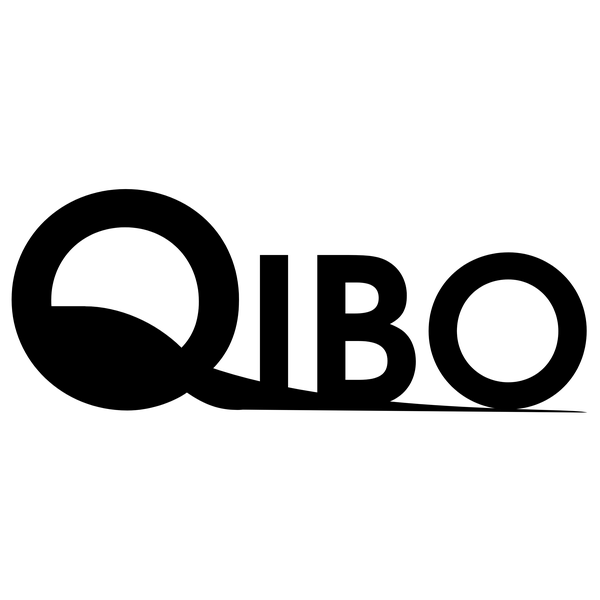
\includegraphics[width=.18\textwidth]{figures/qibo.png} 

\includegraphics[width=.18\textwidth]{figures/unimi.png} 

\includegraphics[width=.18\textwidth]{figures/cern.png}  

\includegraphics[width=.18\textwidth]{figures/qti.png}  
};
\end{tikzpicture}
}

\begin{document}

\maketitle

\begin{frame}{Compute quantum mechanics}
\pause
  \begin{itemize}[noitemsep]
  \item<2,3>[\faGear] Representing $N$ particles is difficult;
  \item<3>[\faGears] considering $N$ spins ($\uparrow, \downarrow$), we deal with a $2^N$ dimensional Hilbert space!
  \end{itemize}
  \vspace{0.5cm}
  \begin{multicols}{2}
    \begin{figure}
       \uncover<2,3>{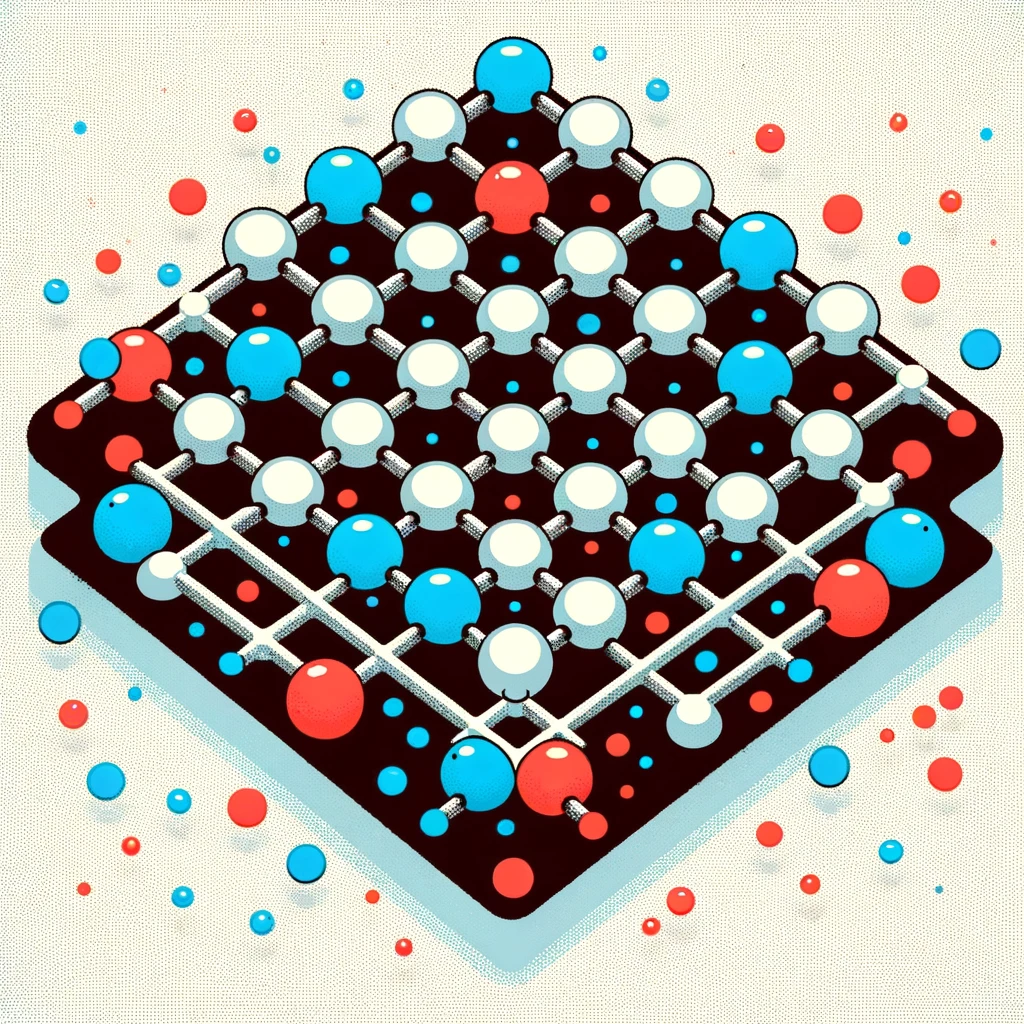
\includegraphics[width=0.45\textwidth]{figures/spins.png}}%
    \end{figure}
    \begin{figure}
       \uncover<3>{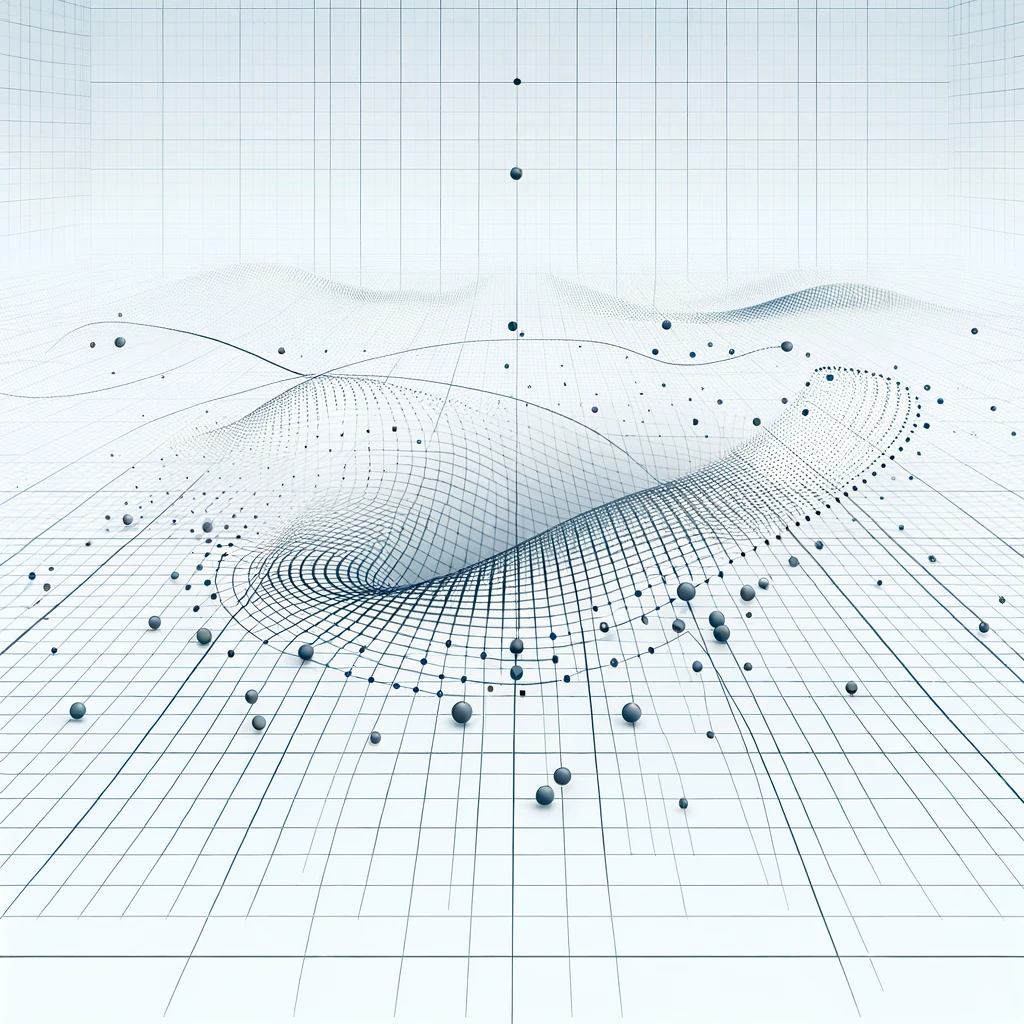
\includegraphics[width=0.45\textwidth]{figures/hilb.png}}%
    \end{figure}
\end{multicols}
\end{frame}

\begin{frame}{What can we do?}
\pause
\begin{itemize}[noitemsep]
\item[1.] we can try to use classical methods to represent the system;
\pause
\item[2.] we can build a quantum computer.
\end{itemize}
\pause
\begin{figure}
   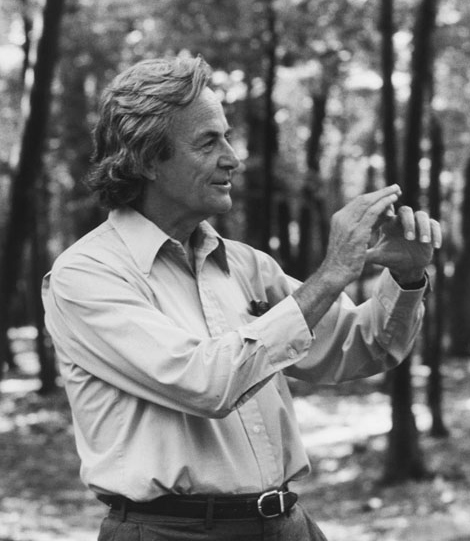
\includegraphics[width=0.4\textwidth, height=0.55\textheight]{figures/feynmann.jpg}%
   $\,\,$ \pause
   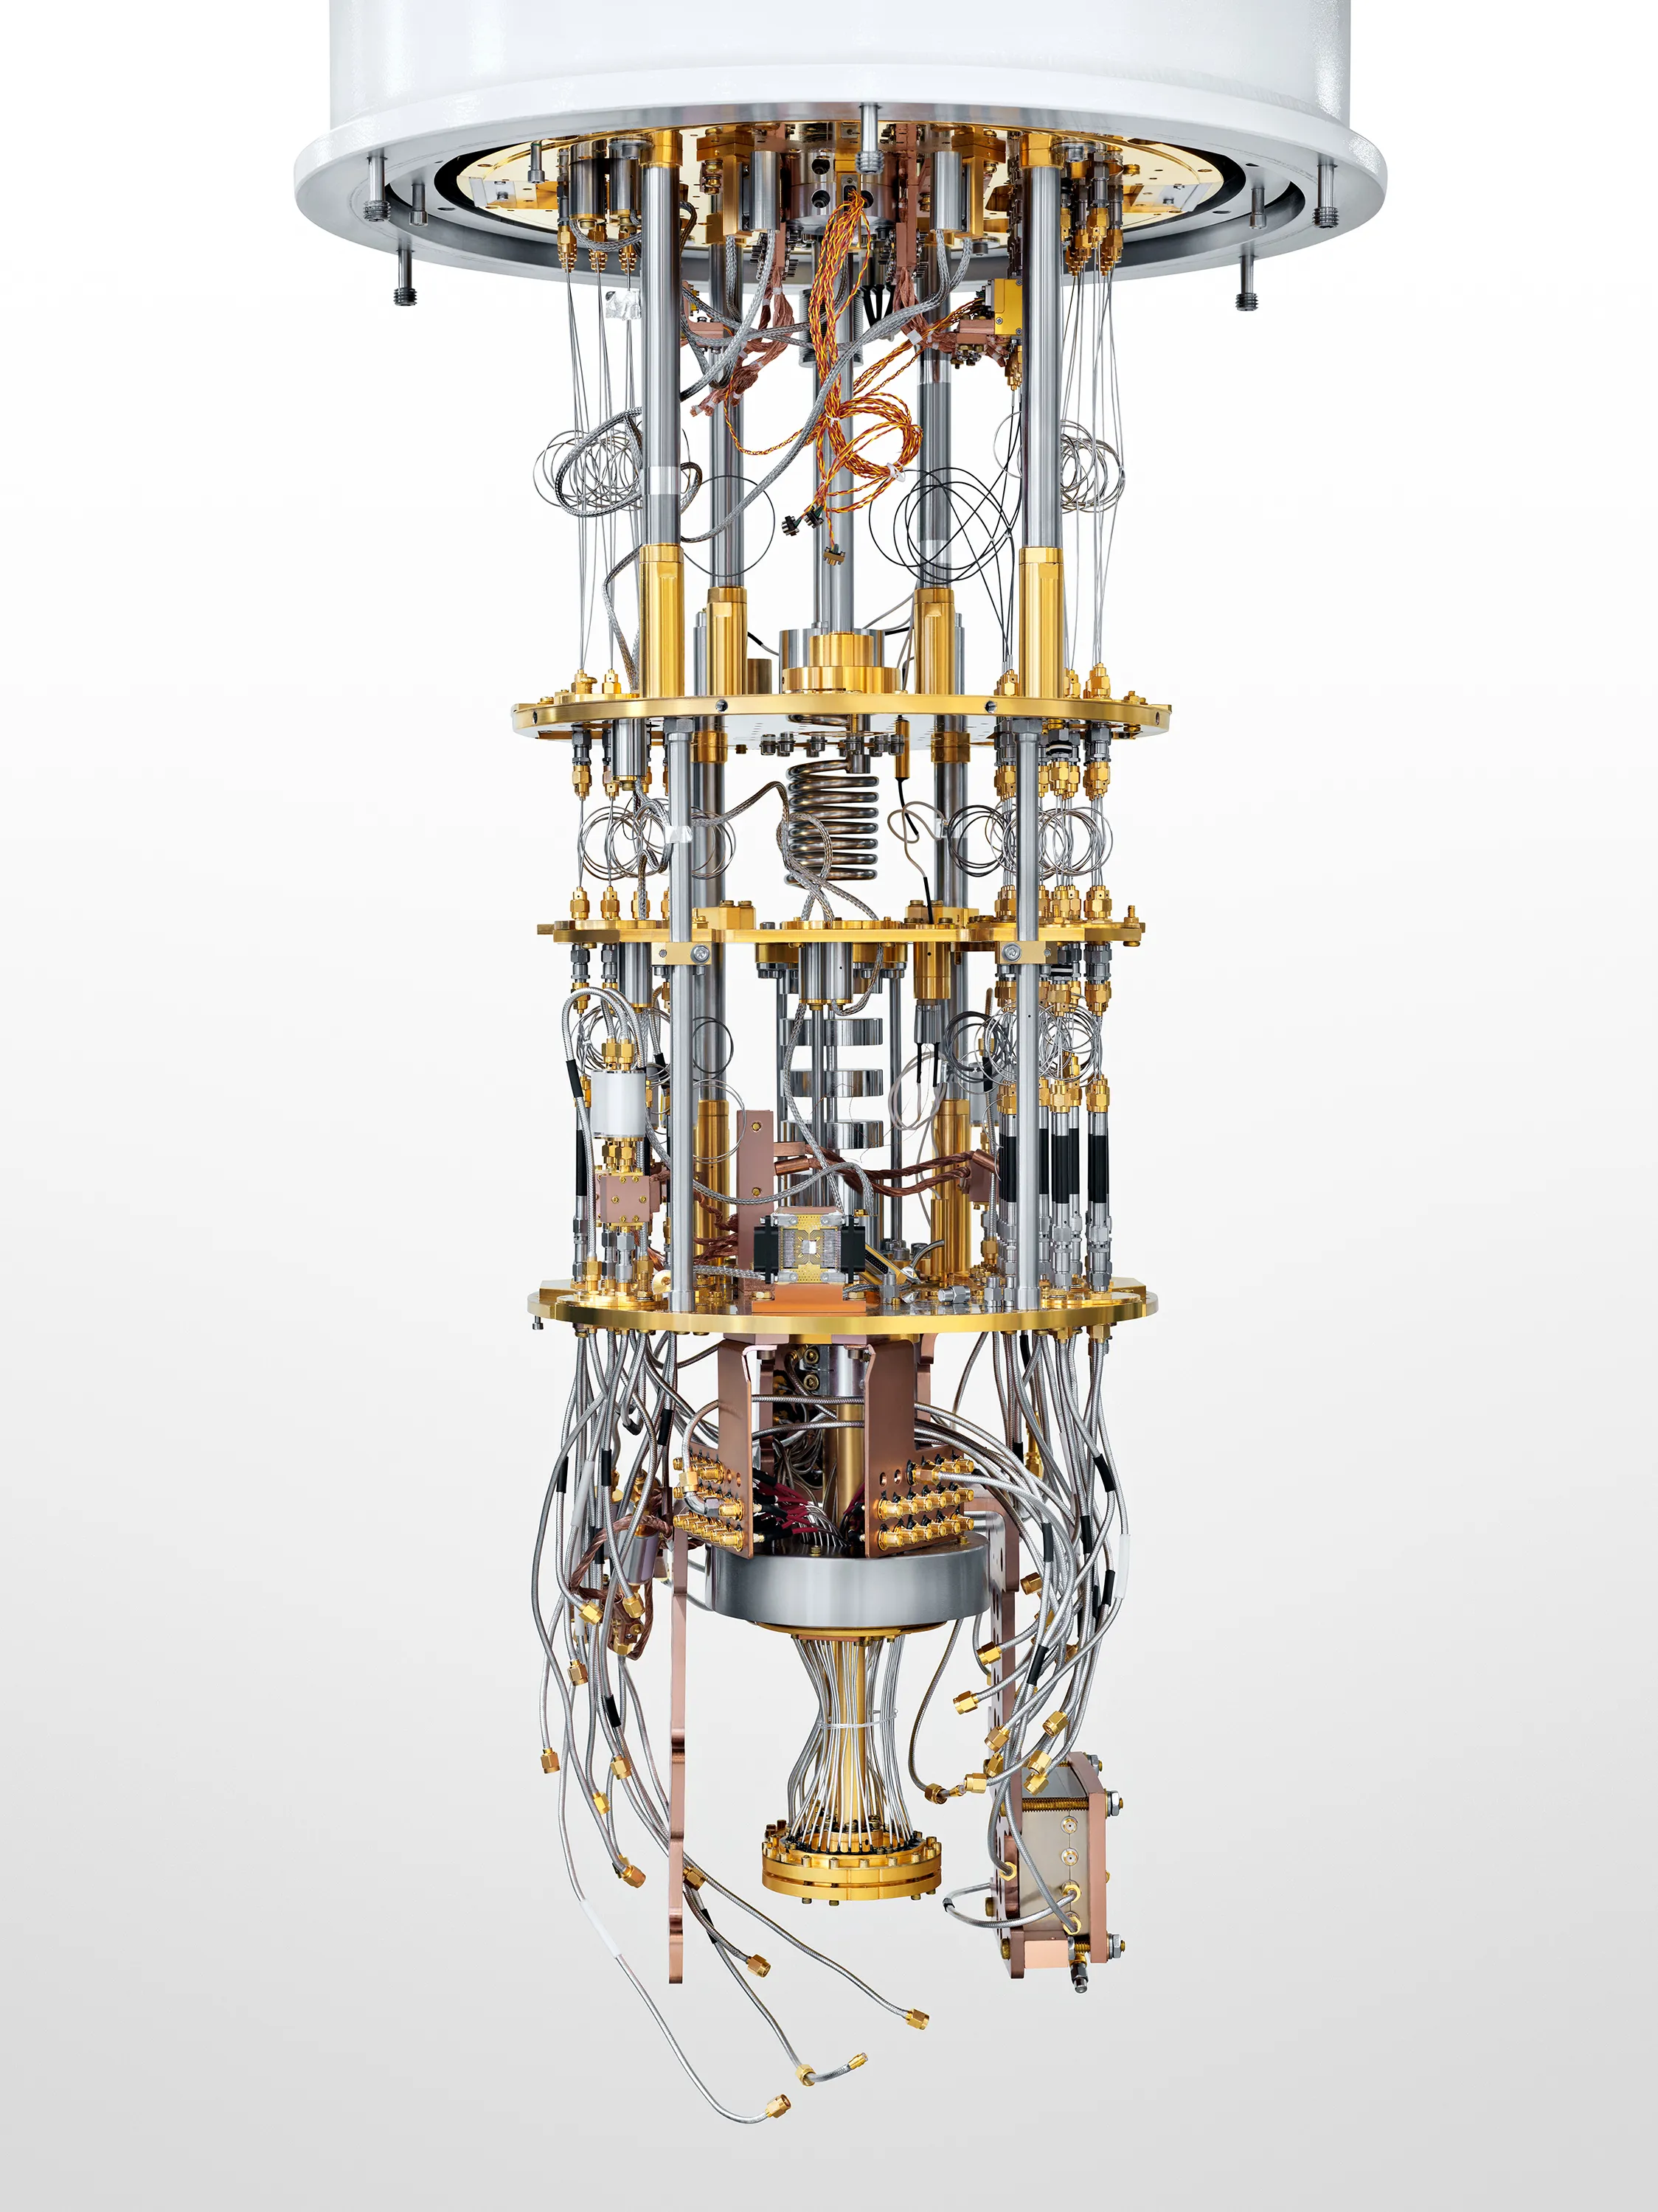
\includegraphics[width=0.4\textwidth, height=0.55\textheight]{figures/qcomp.png}
\end{figure}

\small
\textit{Nature isn't classical, dammit, and if you want to make a simulation of nature, 
you'd better make it quantum mechanical, and by golly it's a wonderful problem, 
because it doesn't look so easy.} 

\href{https://link.springer.com/article/10.1007/BF02650179}{\faBook\,\, Richard Feynman, 1982, Simulating Physics with Computers}
\end{frame}

\begin{frame}{What can we do?}
\begin{itemize}[noitemsep]
\item[1.] \textbf{\textcolor{amethyst}{we can try to use classical methods to represent the system}};
\item[2.] we can build a quantum computer.
\end{itemize}
\begin{figure}
   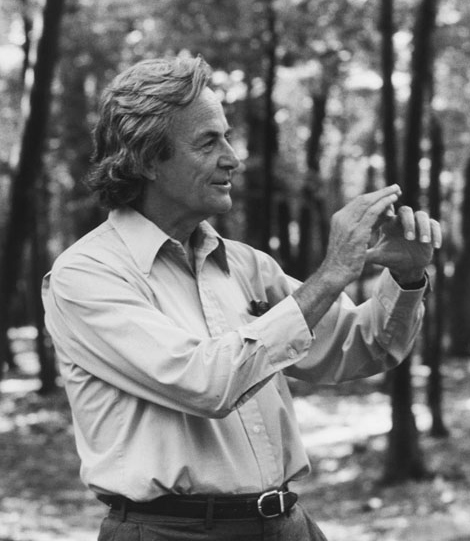
\includegraphics[width=0.4\textwidth, height=0.55\textheight]{figures/feynmann.jpg}%
   $\,\,$ 
   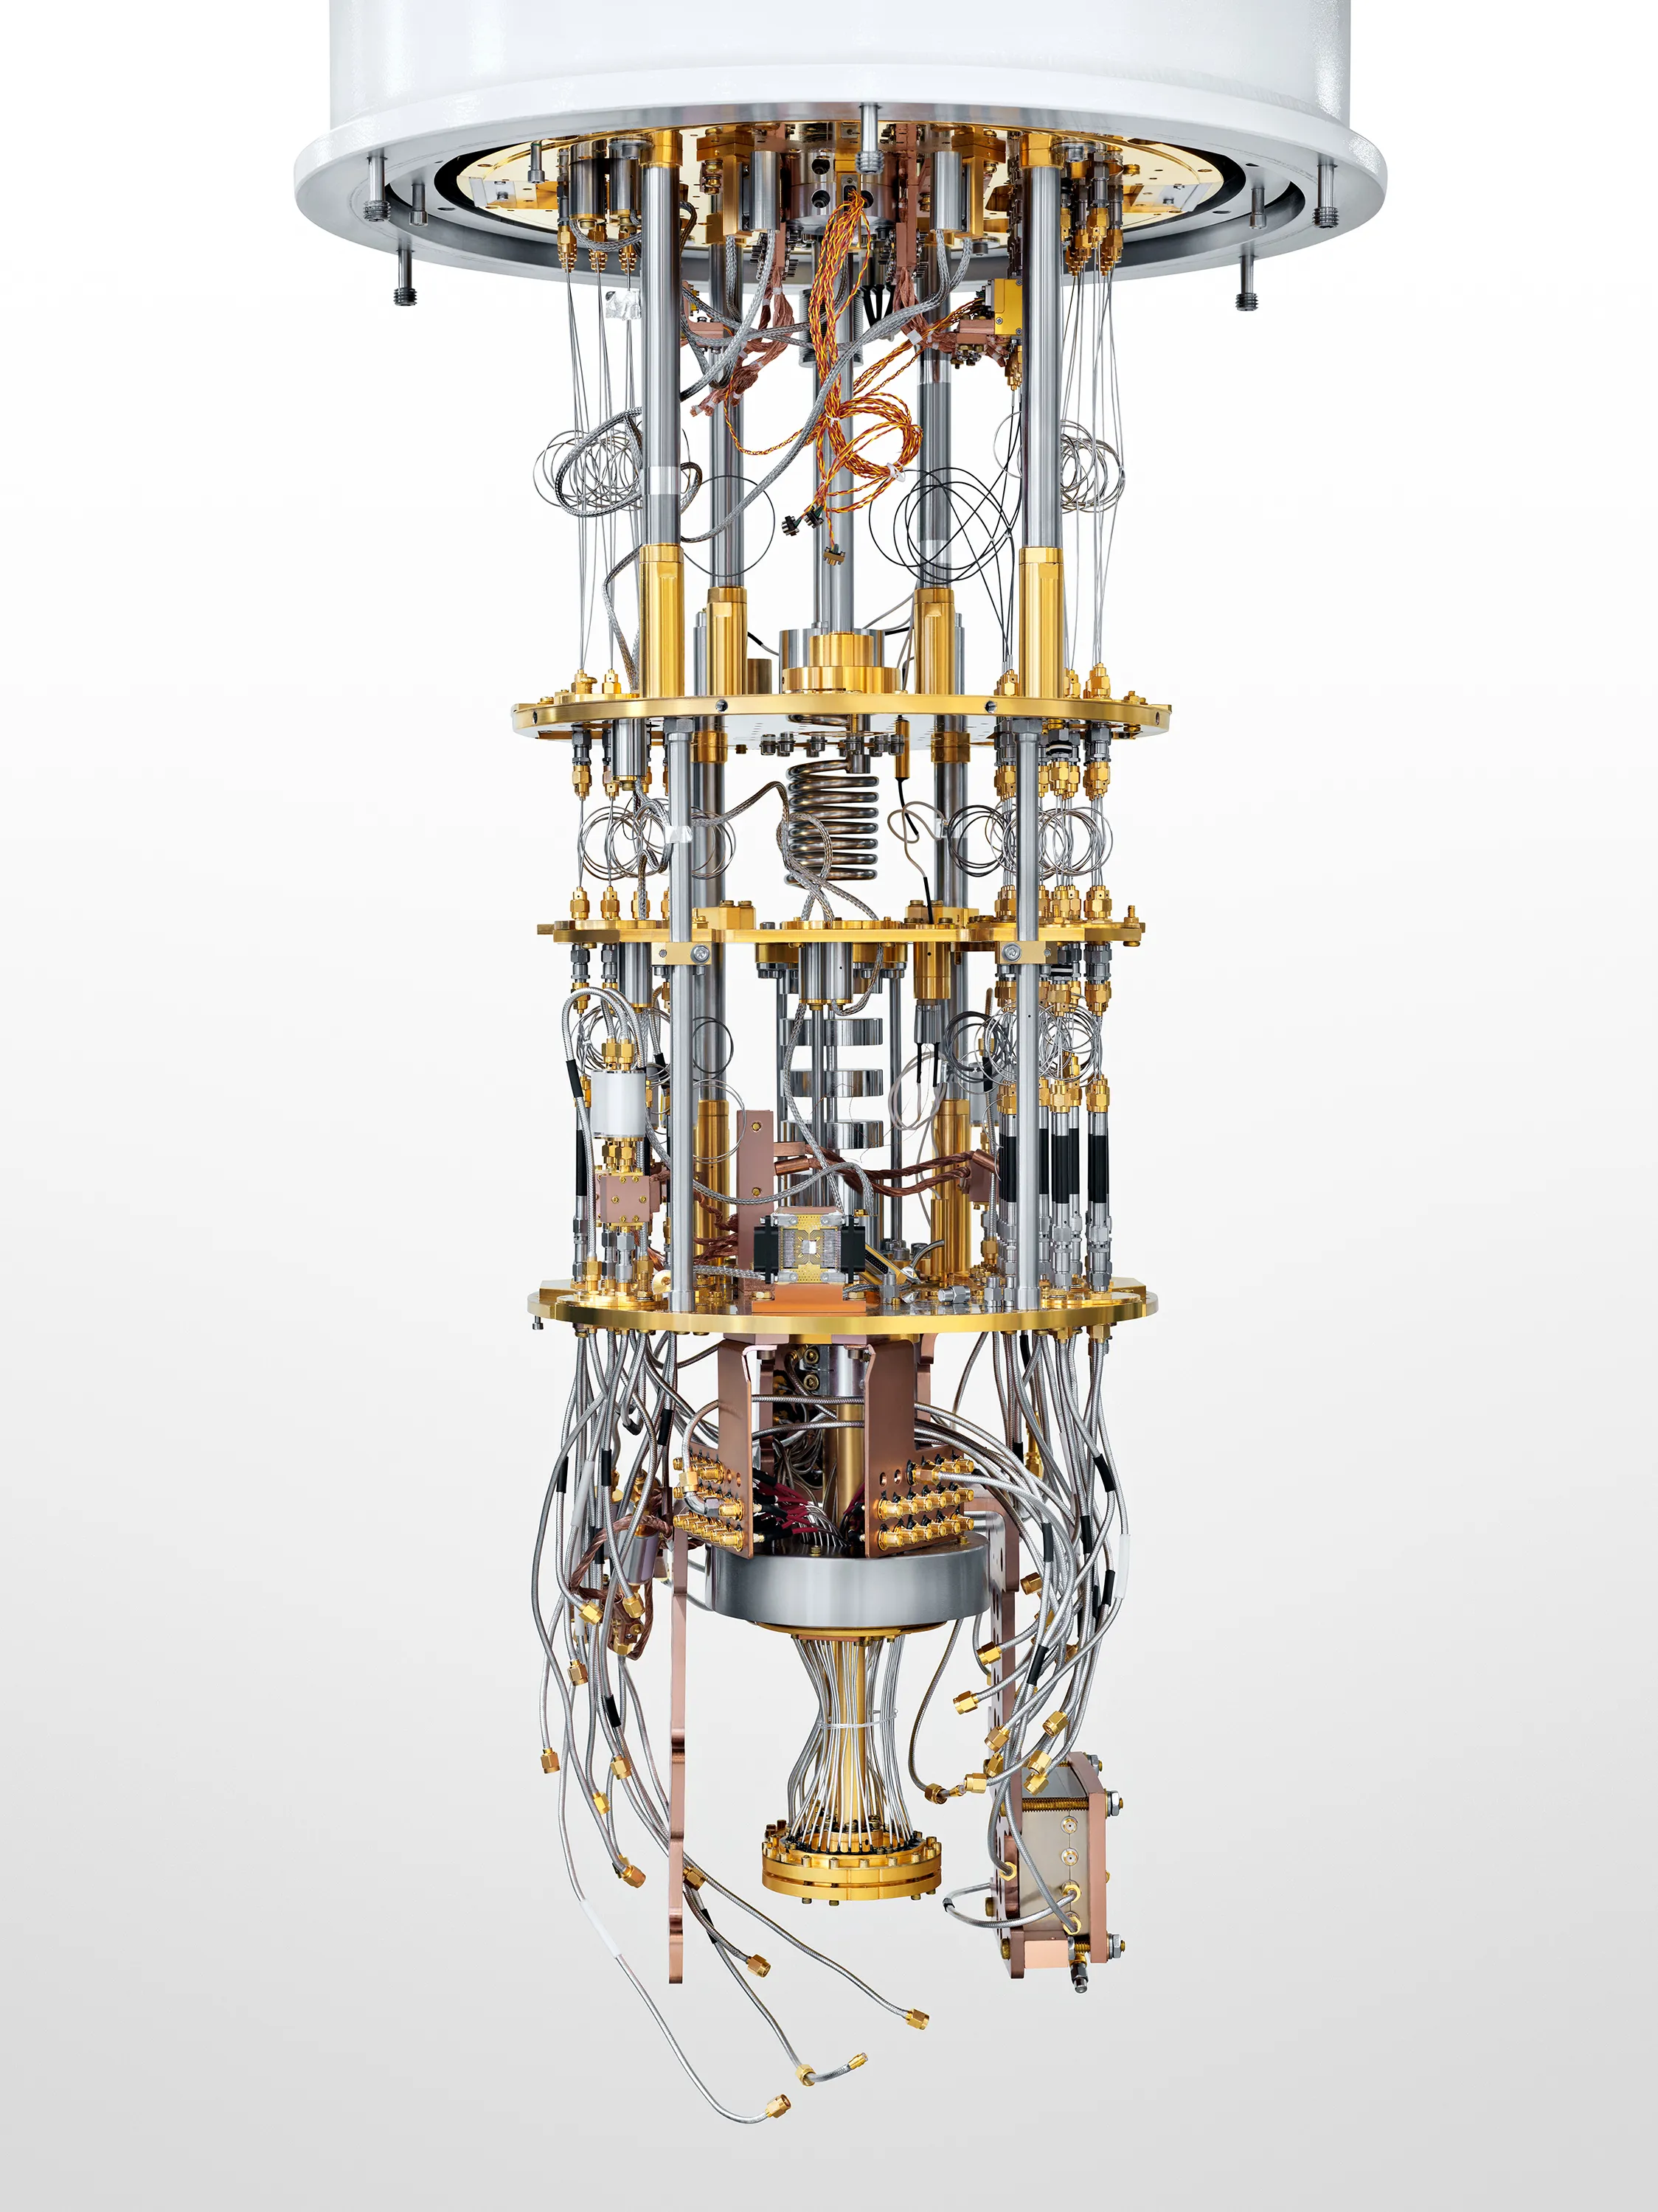
\includegraphics[width=0.4\textwidth, height=0.55\textheight]{figures/qcomp.png}
\end{figure}

\small
\textit{Nature isn't classical, dammit, and if you want to make a simulation of nature, 
you'd better make it quantum mechanical, and by golly it's a wonderful problem, 
because it doesn't look so easy.} 

\href{https://link.springer.com/article/10.1007/BF02650179}{\faBook\,\, Richard Feynman, 1982, Simulating Physics with Computers}
\end{frame}

\begin{frame}{Can we represent a state with a classical computer?}
Let's suppose we want to represent a system of \textbf{qubits} ($\uparrow, \downarrow$).
\pause
\begin{itemize}[noitemsep]
\item[1.] Each \texttt{float 64} requires 8 bytes of memory to be stored;
\pause
\item[2.] each \texttt{complex 128} requires 16 bytes of memory;
\pause
\item[3.] let's take a nice 32Gb of RAM: it can store up to $2$ billions of \texttt{complex 128}.
\pause
\item[4.] a $30$ qubits state requires $\sim 1$ billion of complex numbers;
\pause
\item[5.] a $31$ qubits state cannot be represented by my PC;
\pause
\item[6.] no problem. Let's get serious: \texttt{Fugaku}!
\end{itemize}

\begin{figure}
   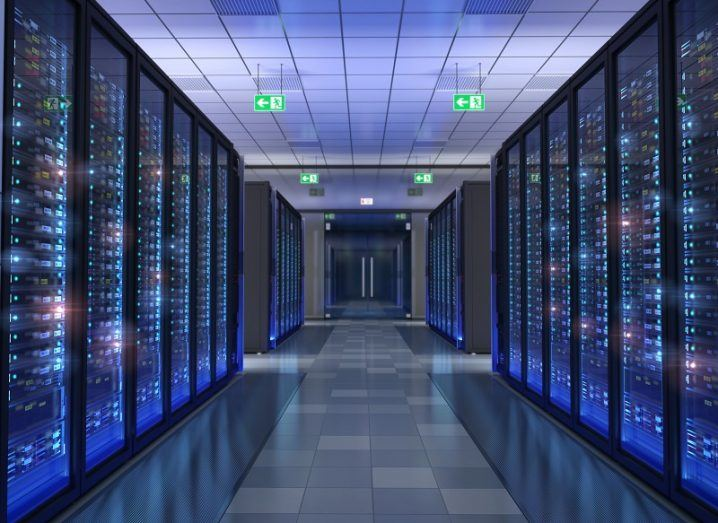
\includegraphics[width=0.48\textwidth, height=0.4\textheight]{figures/fugaku.jpeg}%
   $\,\,$
   \pause
   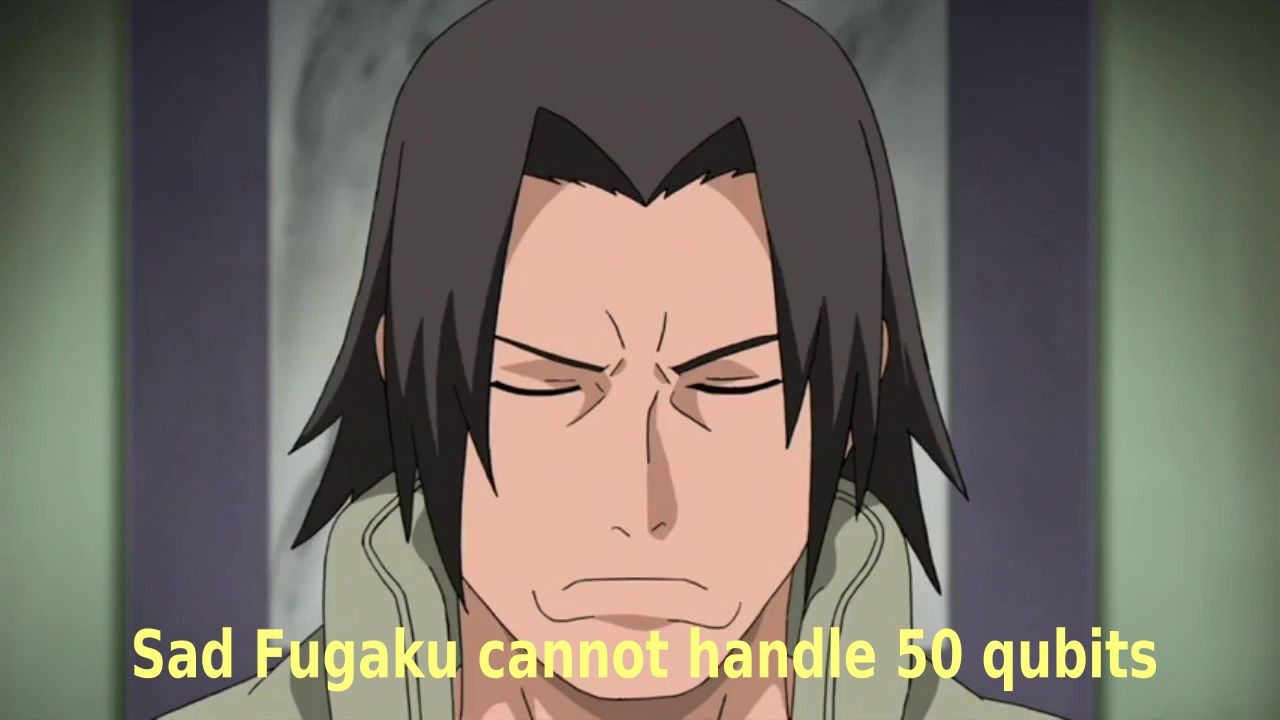
\includegraphics[width=0.48\textwidth, height=0.4\textheight]{figures/sad_fugaku.jpg}
\end{figure}
\end{frame}

\begin{frame}{Some smart strategies}
   \begin{itemize}[noitemsep]
      \item<2,3,4>[1.] Variational Monte Carlo (VMC): given a wave function $\Psi(\bm{x}|\bm{\theta})$ and a target $H$, MC methods are used to minimize:
      $$ \frac{\int \text{d}\bm{x}\, \Psi^*(\bm{x}|\bm{\theta})\, H \, 
      \Psi(\bm{x}|\bm{\theta})}{\int \text{d}\bm{x}\, |\Psi(\bm{x}|\bm{\theta})|^2}\geq E_0; $$
      \item<3,4>[2.] Tensor Networks (TNs): contraction of complex systems into simpler structures;
      \item<4>[3.] Neural Network Quantum States: use complex ANNs to represent the state.
   \end{itemize}
   \begin{multicols}{3}
   \begin{figure}
      \uncover<2,3,4>{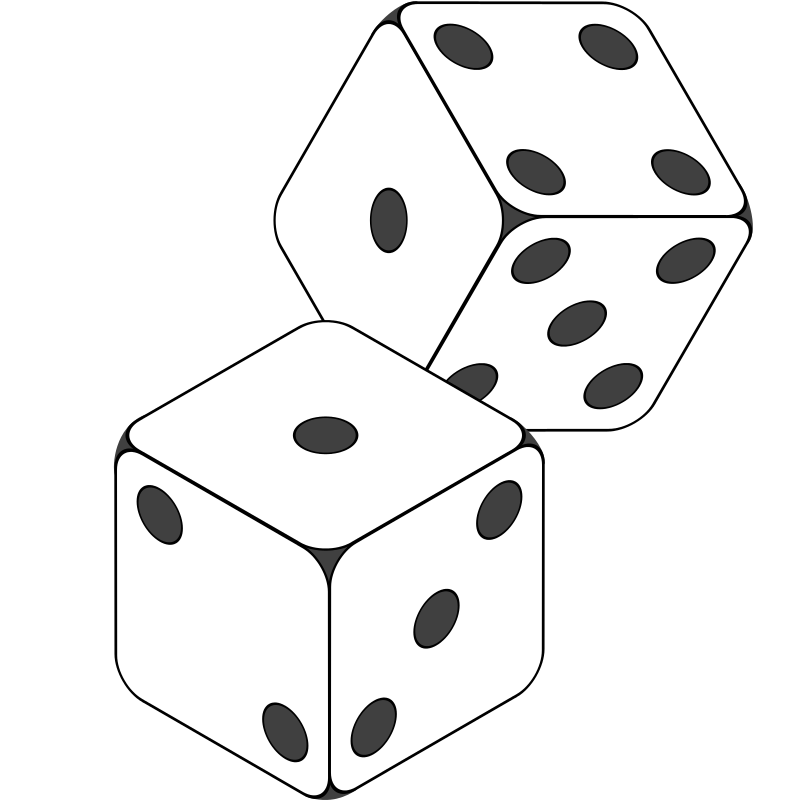
\includegraphics[width=0.9\linewidth, height=0.35\textheight]{figures/dices.png}
      \caption*{\href{https://arxiv.org/abs/1508.02989}{\faBook\,\,arXiv:1508.02989}}}%
      \uncover<3,4>{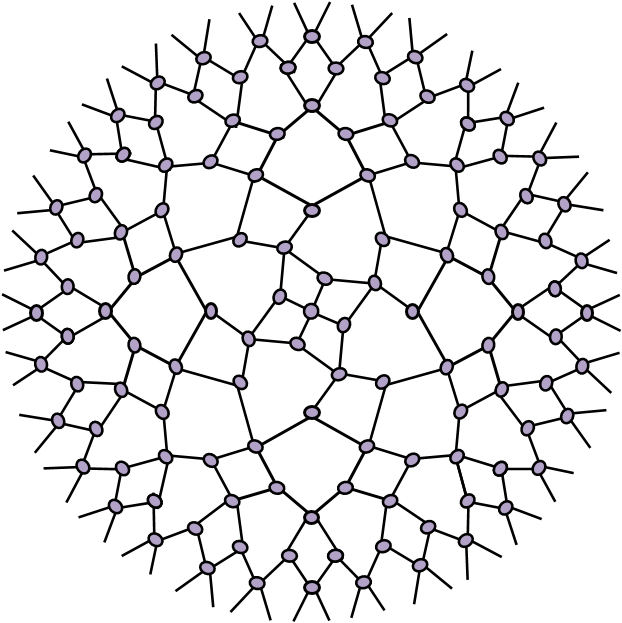
\includegraphics[width=0.9\linewidth, height=0.35\textheight]{figures/tn.png}
      \caption*{\href{https://arxiv.org/abs/1708.00006}{\faBook\,\,arXiv:1708.00006}}}%
      \uncover<4>{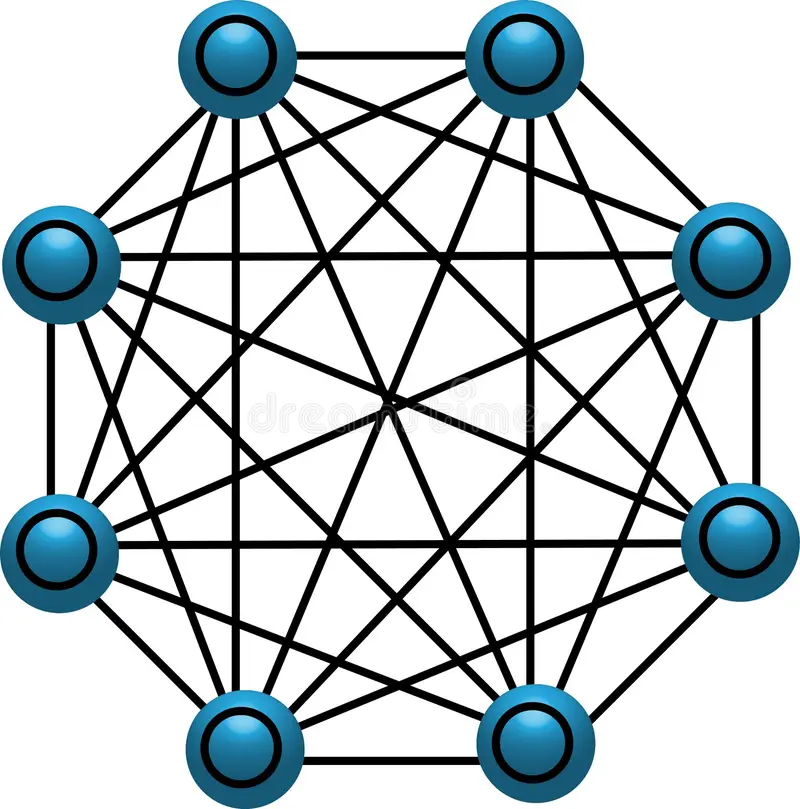
\includegraphics[width=0.9\linewidth, height=0.35\textheight]{figures/bm.png}
      \caption*{\href{https://arxiv.org/abs/1606.02318}{\faBook\,\,arXiv:1606.02318}}}
   \end{figure}   
   \end{multicols}
\end{frame}

\section{A snapshot of quantum computing}

\begin{frame}{Qubits}
        \begin{itemize}[noitemsep]
           \item<2,3,4,5>[1.] classical bits are replaced by \textbf{qubits}
           $ \ket{\psi} = \alpha\ket{0}+\beta\ket{1}$.
           \item<3,4,5>[2.] we can manipulate the qubit state applying \textbf{gates}: $\ket{\psi'}=\mathcal{U}(\bm{\theta})\ket{\psi}.$

           Typically we use 1-qubit and 2-qubits gates!
         %   $$ H \ket{0} = \frac{\ket{0}+\ket{1}}{\sqrt{2}} \qquad \text{with}\qquad  H = 
         %   \begin{pmatrix}
         %   1 & 1 \\ 1 & -1
         %   \end{pmatrix}.
         %   $$
           \item<4,5>[3.] combine together gates to build \textbf{quantum circuits};
           \item<5>[4.] to access the information we need to measure the system.
        \end{itemize}
        \begin{figure}
            \only<2>{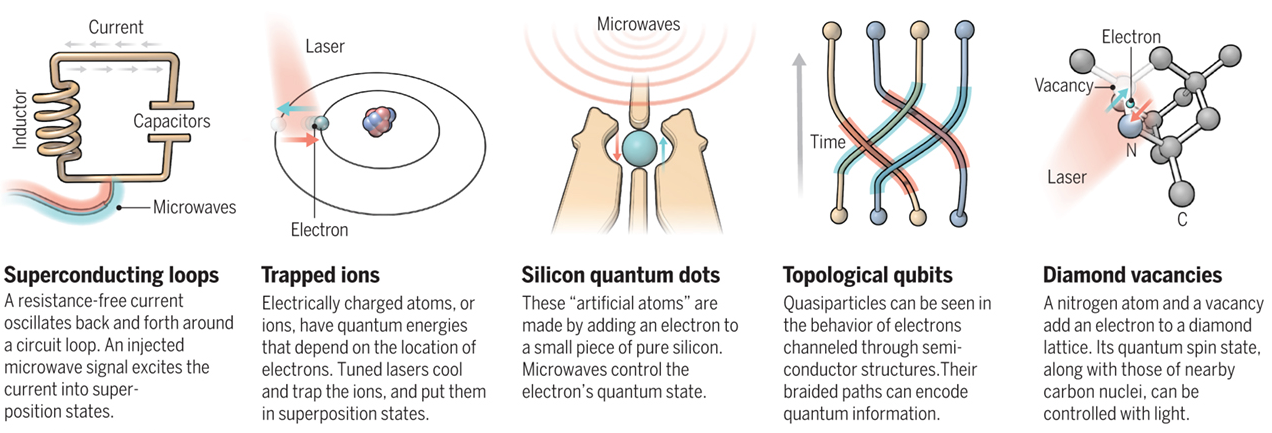
\includegraphics[width=0.95\linewidth, height=0.45\textheight]{figures/qubits.png}}%
            \only<3>{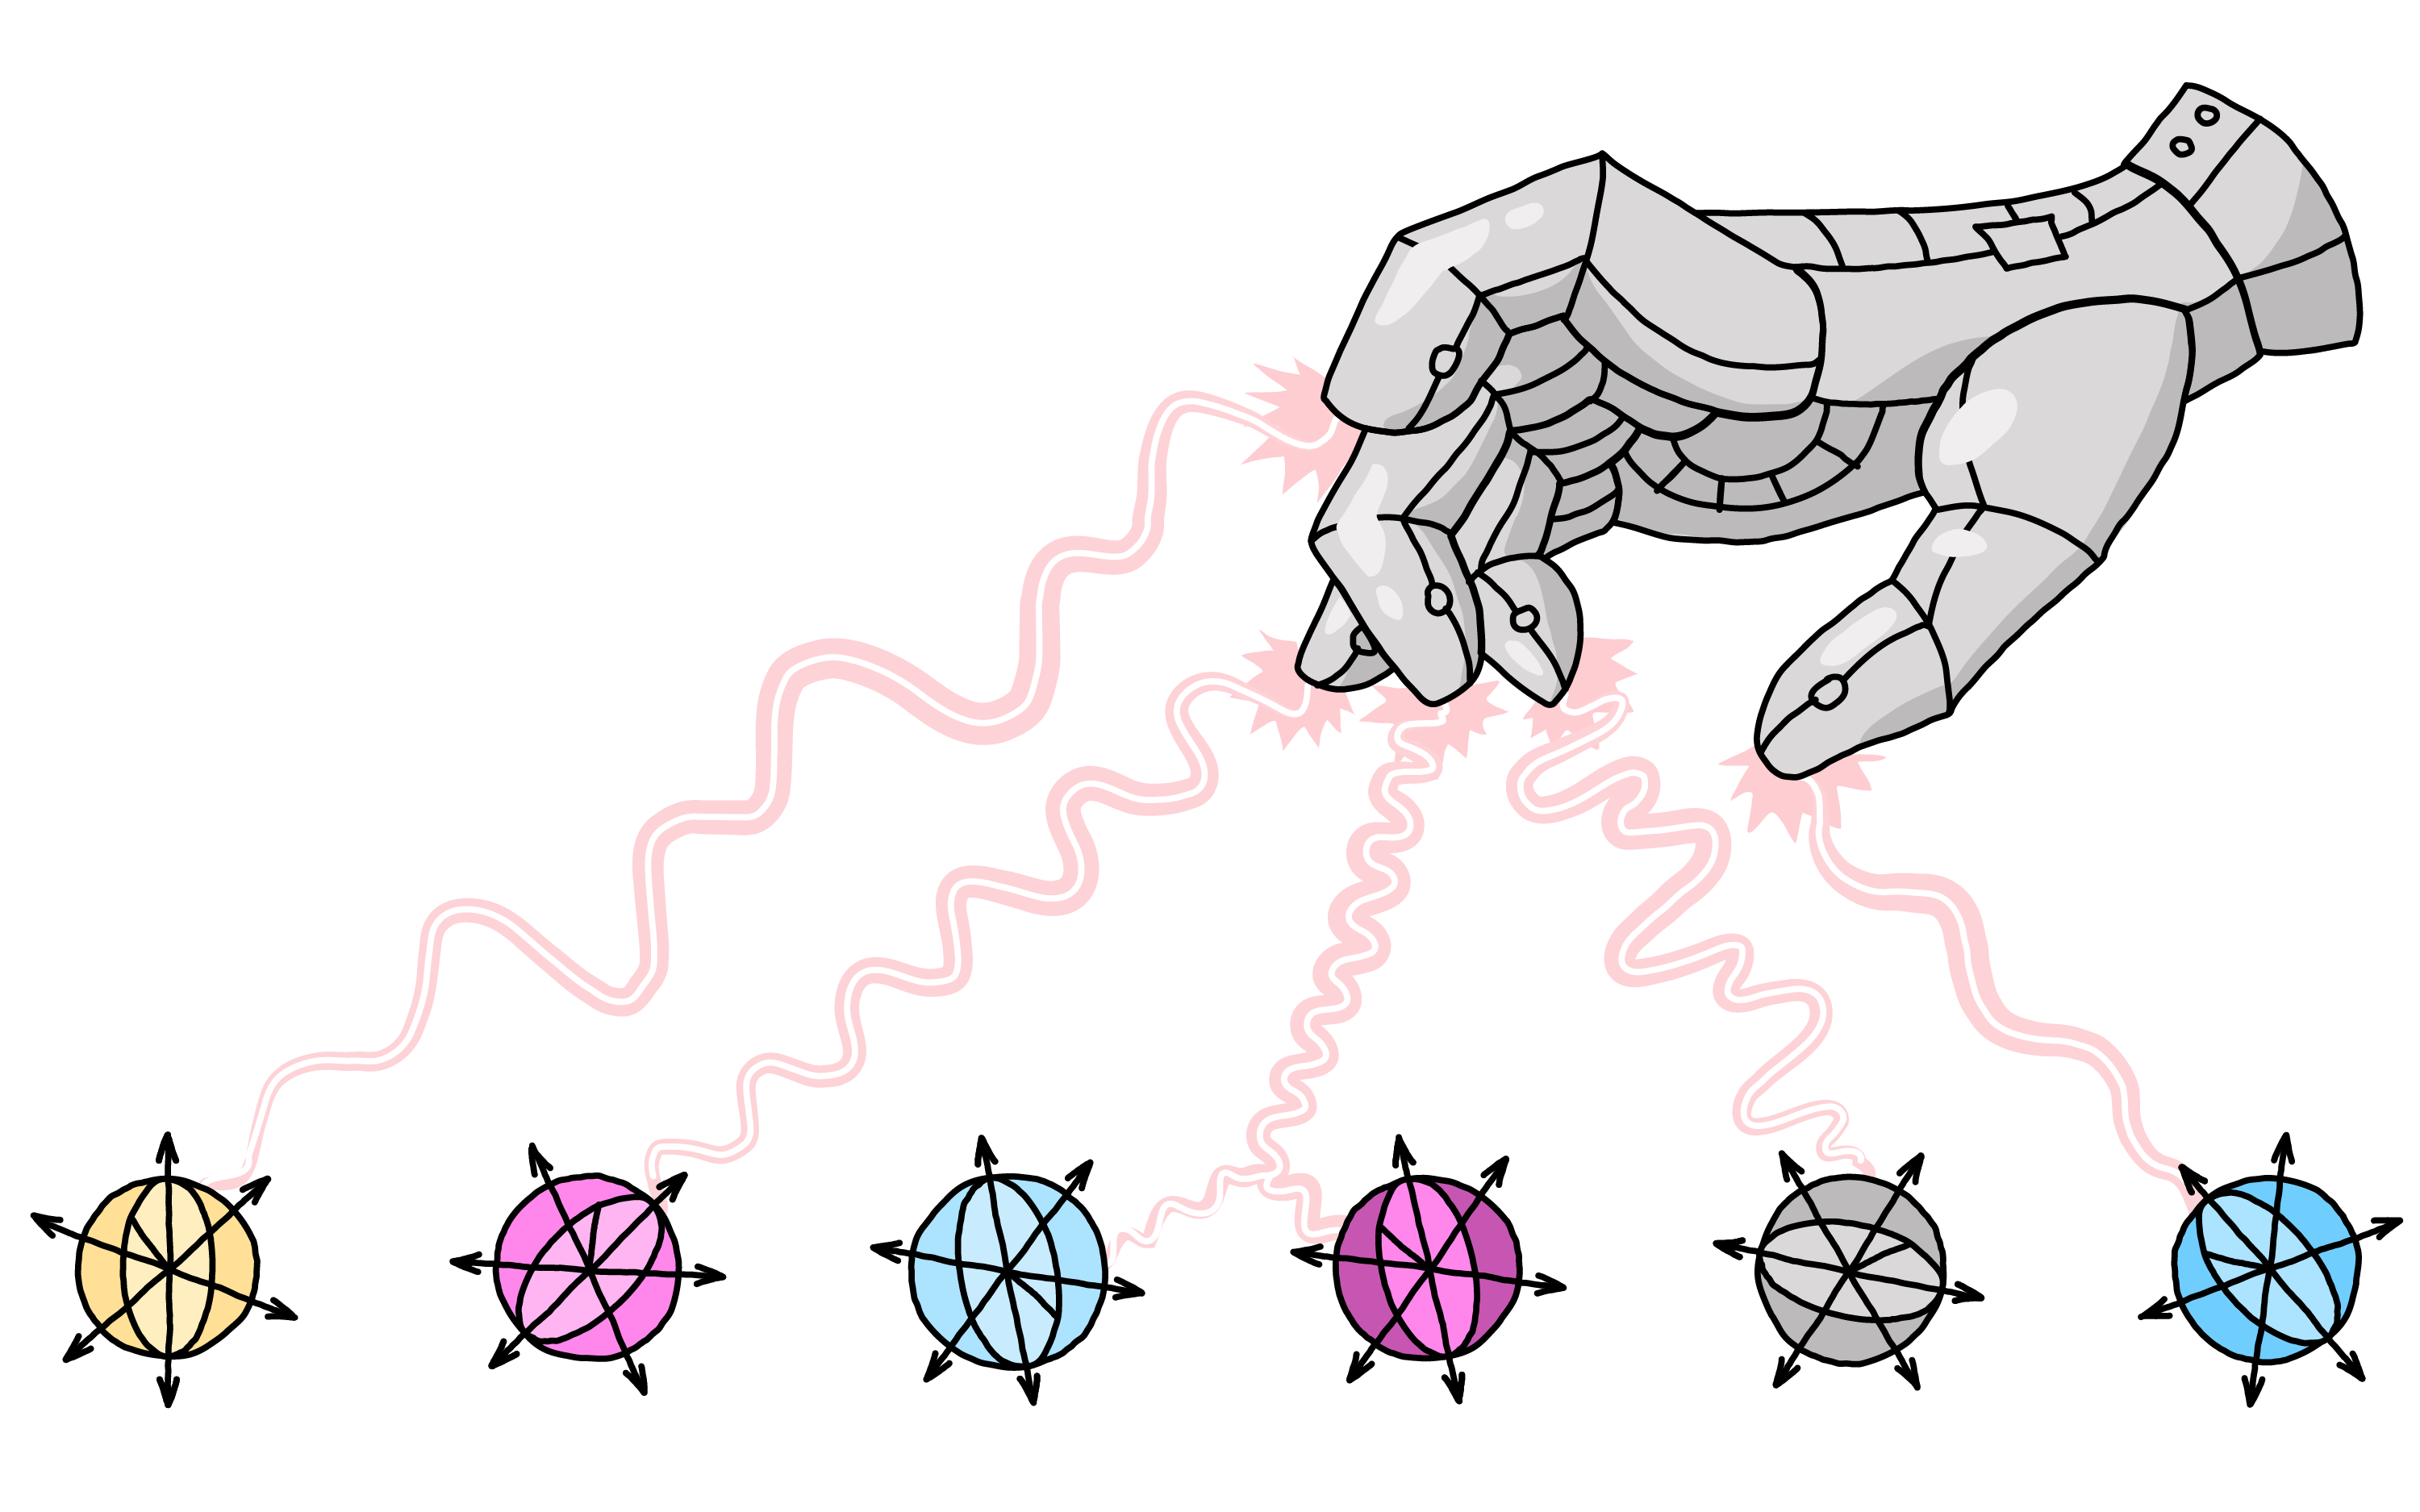
\includegraphics[width=0.5\linewidth, height=0.45\textheight]{figures/pulses.png}}%
            \only<4>{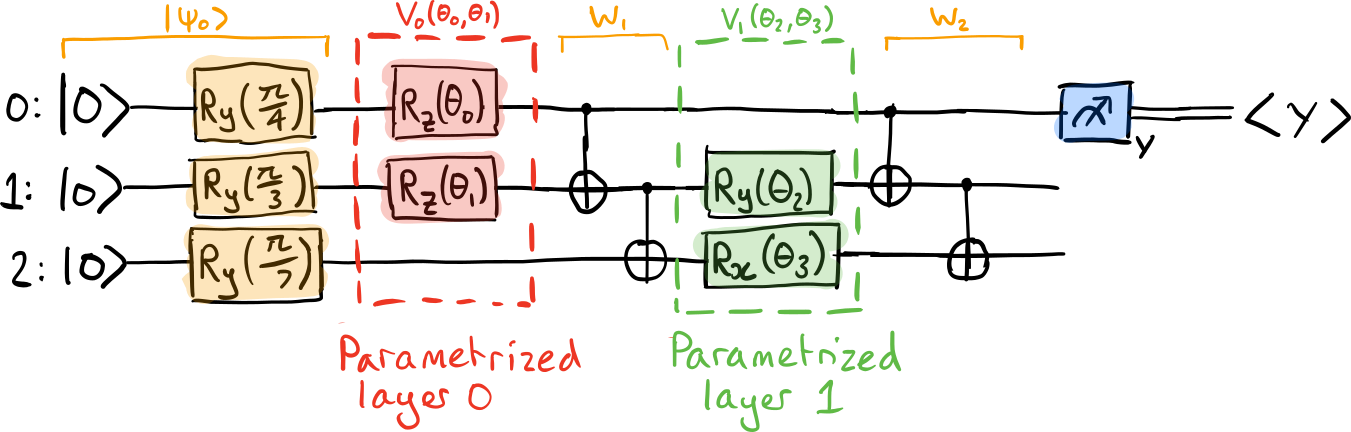
\includegraphics[width=0.9\linewidth, height=0.45\textheight]{figures/circuit.png}}
            \only<5>{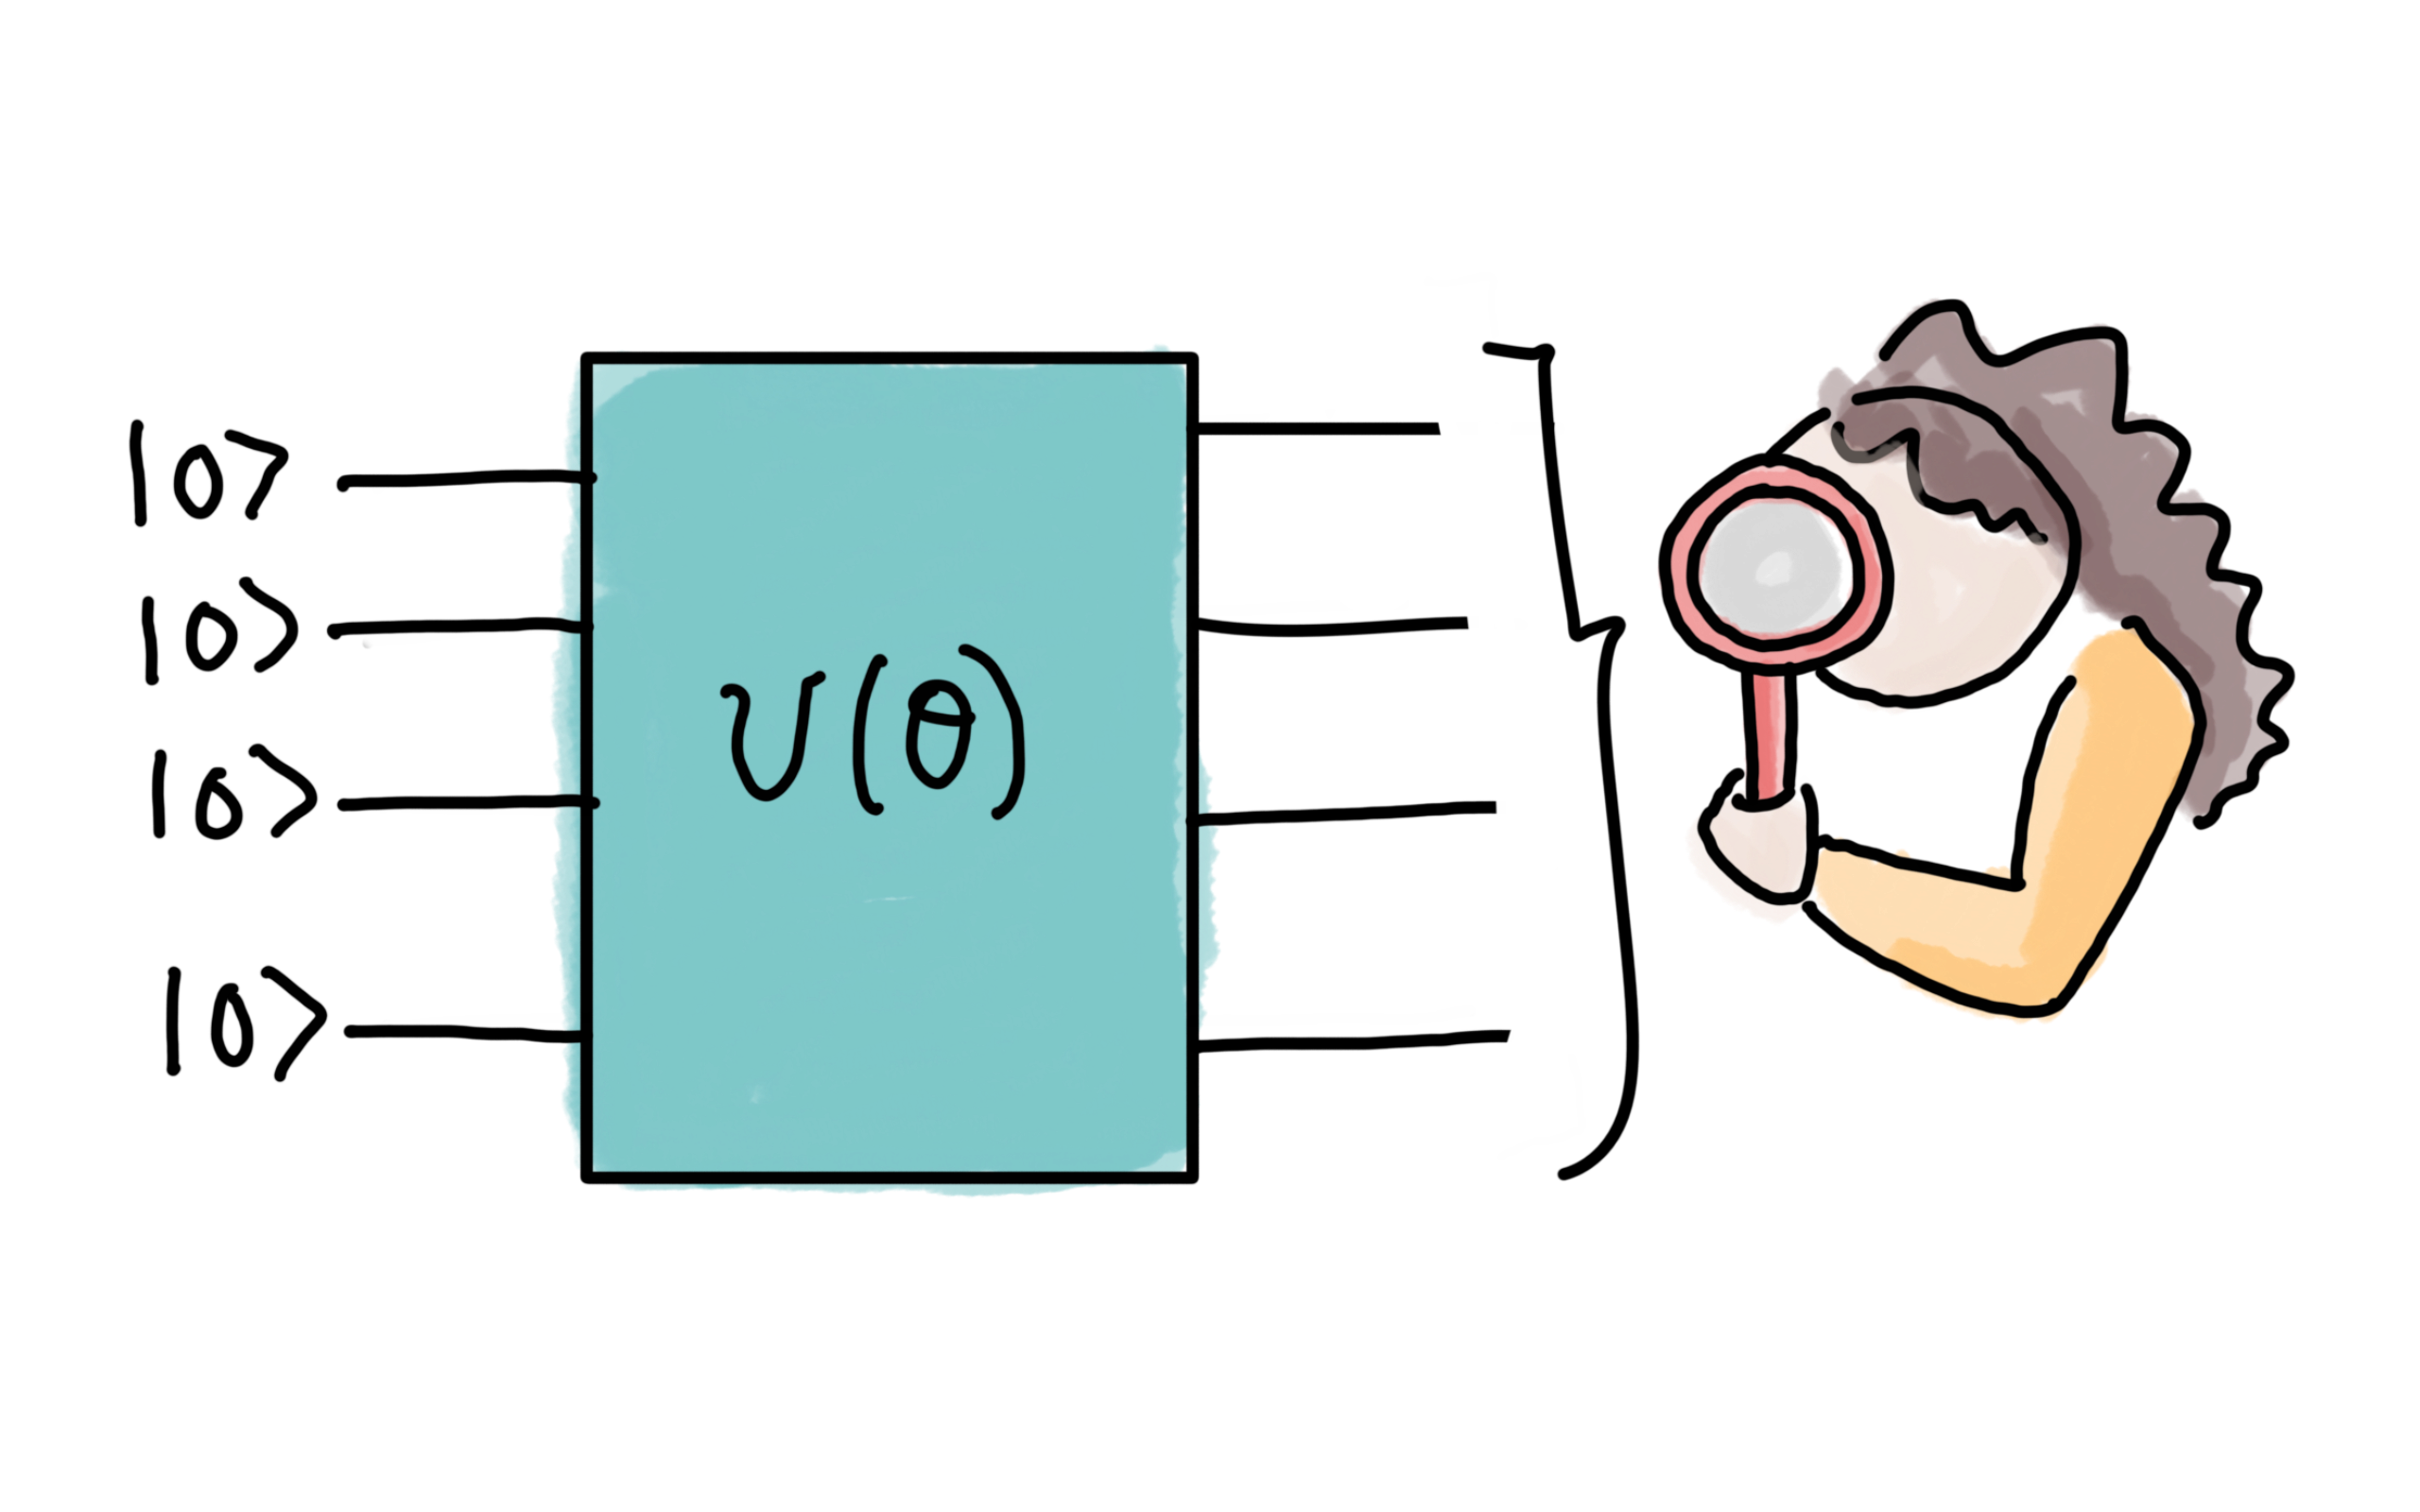
\includegraphics[width=0.7\linewidth, height=0.45\textheight]{figures/measurement.png}}
        \end{figure}        
\end{frame}


\begin{frame}{New computational power}
\pause
With quantum computing, we introduce new tools.
\pause
\begin{itemize}[noitemsep]
\item[\faRocket] prepare a quantum state in the computational zero $\ket{0}$;
\pause
\item[\faSliders] we can prepare superposition: 
$$H\ket{0} = \frac{1}{\sqrt{2}}(\ket{0} + \ket{1}) \pause \quad \text{with} \quad H = \frac{1}{\sqrt{2}}
\begin{bmatrix} 1 & 1 \\ 1 & -1 \end{bmatrix},\,\, \ket{0}=\begin{bmatrix} 1 \\ 0 
\end{bmatrix},\,\,\ket{1}=\begin{bmatrix} 0 \\ 1 \end{bmatrix};$$
\pause
\item[\faShareAlt] let's apply a controlled-NOT (CNOT) gate on a second qubit prepared in $\ket{0}$:
$$ \text{CNOT} \biggl( \underbrace{\frac{1}{\sqrt{2}}(\ket{0} + \ket{1})}_{\text{control}}\otimes 
\ket{0} \biggr) = \pause \frac{1}{\sqrt{2}}(\ket{\textcolor{bleudefrance}{0}0} + 
\text{NOT}_{\rm targ}\ket{\textcolor{brightmaroon}{1}0}) = \pause \frac{1}{\sqrt{2}}(\ket{00} + \ket{11}). $$
\end{itemize}
\pause
\begin{figure}
   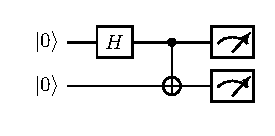
\includegraphics[width=0.6\linewidth]{figures/baby3.pdf}
\end{figure}    
\end{frame}

\section{Quantum Machine Learning}

\begin{frame}{Classical Machine Learning}
\pause
I asked ChatGPT to give me a comprehensive diagram of Machine Learning (ML) models.
\begin{figure}
   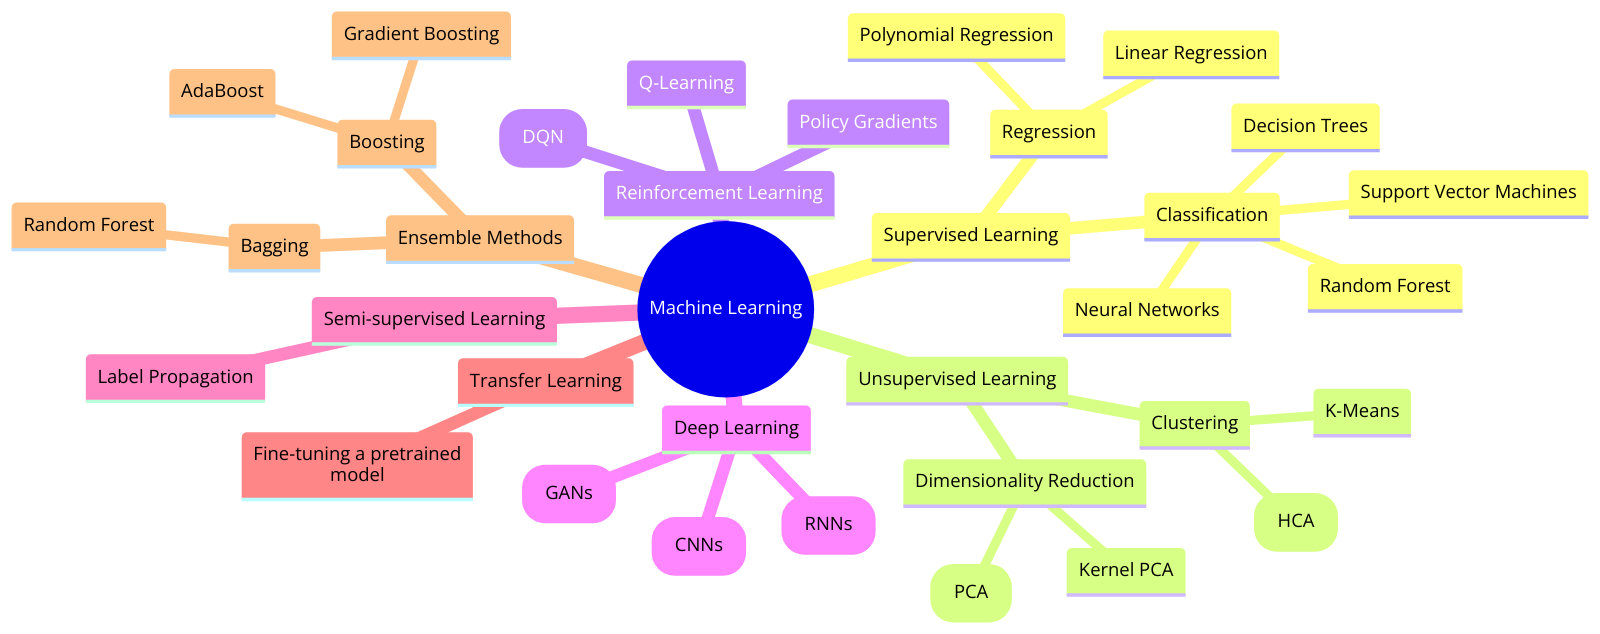
\includegraphics[width=1\linewidth, height=0.5\textheight]{figures/ml.png}
\end{figure}  
\textcolor{white}{Focusing on the supervised ML:}
\begin{itemize}[noitemsep]
\item[] \textcolor{white}{we aim to know some hidden law between two variables: $\bm{y}=f(\bm{x})$}
\item[] \textcolor{white}{we define a parameteric model which returns $\bm{y}_{\rm est}=f_{\rm est}(\bm{x}; \bm{\theta})$}
\item[] \textcolor{white}{we define an optimizer, which task is to compute} 
   \textcolor{white}{$\text{argmin}_{\bm{\theta}}\bigl[J(\bm{y}_{\rm meas}, \bm{y}_{\rm est})\bigr]$}
\end{itemize}
\end{frame}

\begin{frame}{Classical Machine Learning}
I asked ChatGPT to give me a comprehensive diagram of Machine Learning (ML) models.
\begin{figure}
   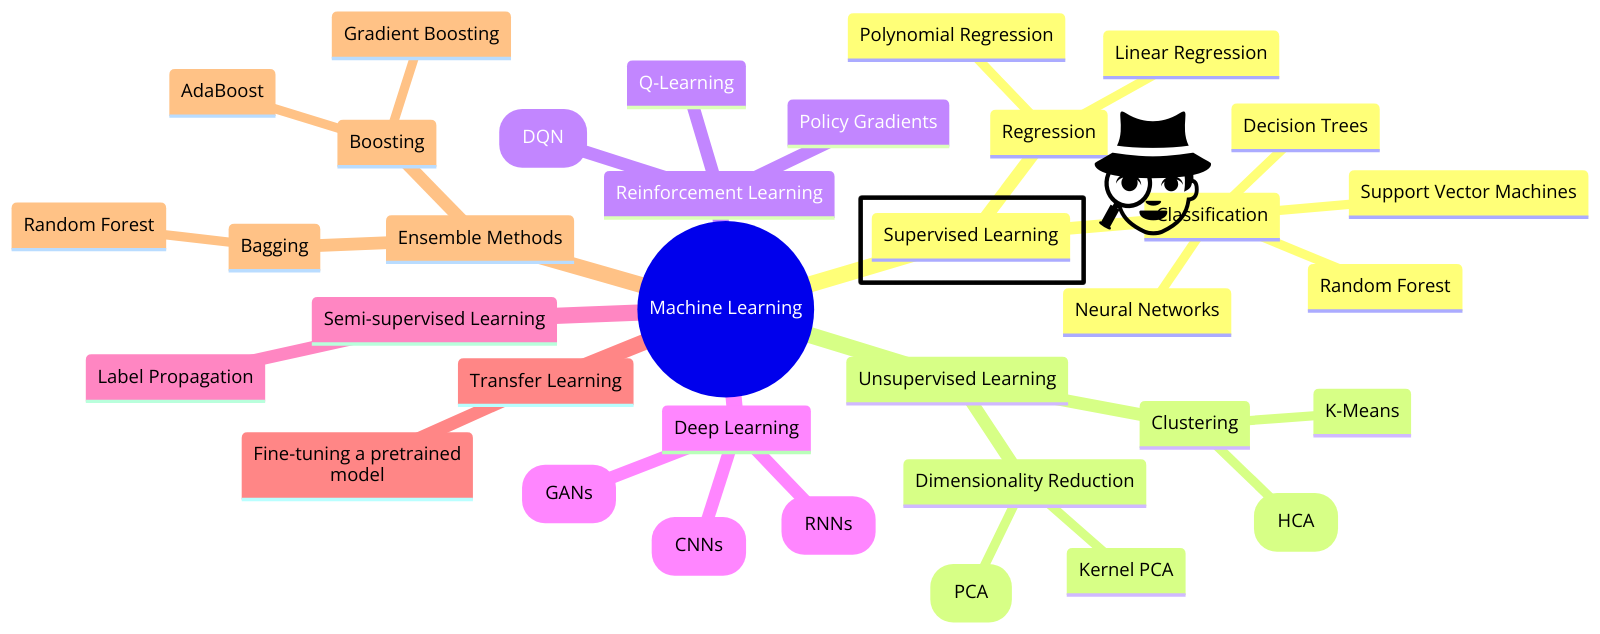
\includegraphics[width=1\linewidth, height=0.5\textheight]{figures/supervised.png}
\end{figure}  
Focusing on the supervised ML!
\pause
\begin{itemize}[noitemsep]
\item[\faCrosshairs] we aim to know some hidden law between two variables: $\bm{y}=f(\bm{x})$;
\pause
\item[\faBarChart] we define a parameteric model which returns $\bm{y}_{\rm est}=f_{\rm est}(\bm{x}; \bm{\theta})$;
\pause
\item[\faBinoculars] we define an optimizer, which task is to compute 
   $\text{argmin}_{\bm{\theta}}\bigl[J(\bm{y}_{\rm meas}, \bm{y}_{\rm est})\bigr]$.
\end{itemize}
\end{frame}

\begin{frame}{Classical Machine Learning}
\begin{figure}
   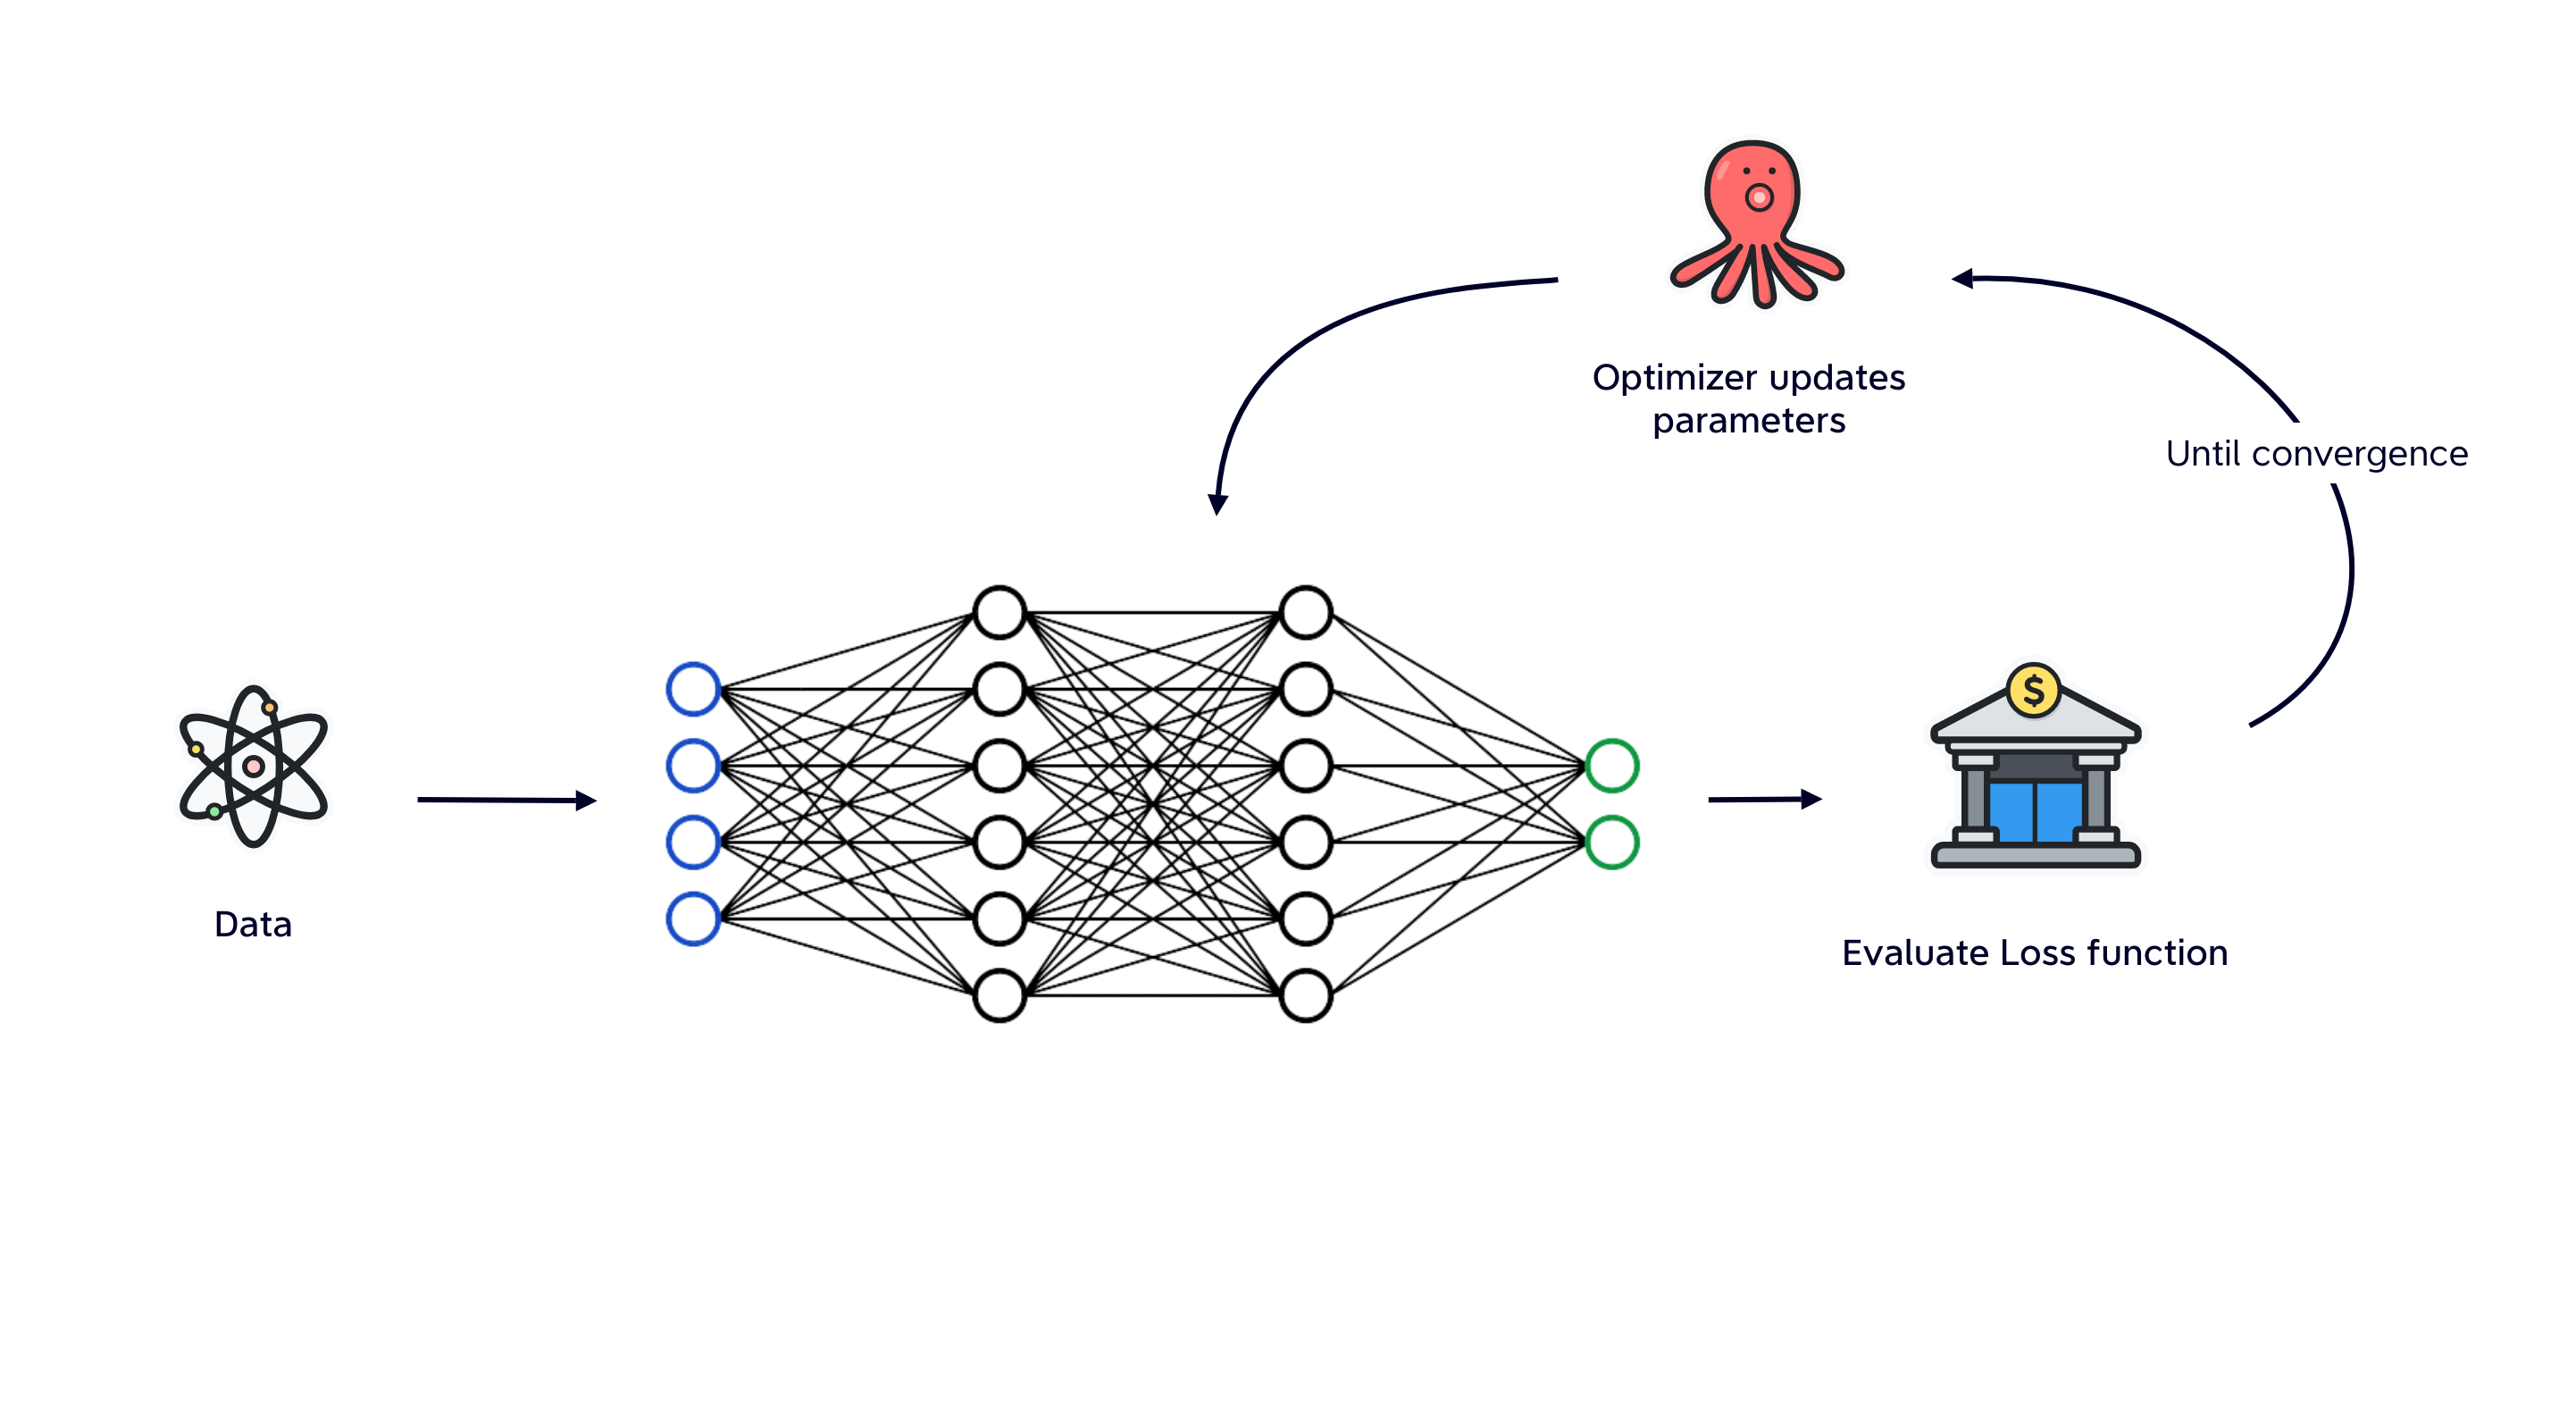
\includegraphics[width=1\linewidth]{figures/ml_scheme.png}
\end{figure}  
\end{frame}

\begin{frame}{Parametric gates}
\pause
\begin{itemize}[noitemsep]
\item[\faLightbulbO] Among the gates, parametric ones can be useful!
\pause
\item[\faMapPin] Let's consider a single qubit system:
\begin{equation*}
   \ket{\psi} = \alpha\ket{0}+\beta\ket{1} \qquad \pause \text{with} 
   \qquad \alpha = \cos{\frac{\theta}{2}}, \quad \beta = e^{i\phi}\sin{\frac{\theta}{2}}.
\end{equation*}
\end{itemize}
\begin{multicols}{2}
\def\rotationSphere{-110}
\def\radiusSphere{2cm}
\def\psiLat{45}
\def\psiLon{45}
\begin{blochsphere}[radius=\radiusSphere,opacity=0,rotation=\rotationSphere]
  % \drawBallGrid[style={opacity=.3}]{30}{45}
  % Draw the sphere...
  \drawLongitudeCircle[]{\rotationSphere}

  \drawLatitudeCircle[style={dashed}]{0}
  % Define the different points on the bloch sphere
  \labelLatLon{ket0}{90}{0};
  \labelLatLon{ket1}{-90}{0};
  \labelLatLon{ketminus}{0}{180};
  \labelLatLon{ketplus}{00}{0};
  \labelLatLon{ketpluspi2}{0}{-90};  % Longitude seems to be defined in the "wrong" direction, hence the minus
  \labelLatLon{ketplus3pi2}{0}{-270};
  \labelLatLon{psi}{\psiLat}{-\psiLon};
  % Draw and label the axis
  \draw[-latex] (0,0) -- (ket0) node[above,inner sep=.5mm] at (ket0) {\footnotesize $z$};
  \draw[-latex] (0,0) -- (ketplus) node[below,inner sep=.5mm] at (ketplus) {\footnotesize$x$};
  \draw[-latex] (0,0) -- (ketpluspi2) node[below,inner sep=.5mm] at (ketpluspi2) {\footnotesize $y$};
  % Draw |psi>
  \draw[-latex] (0,0) -- (psi) node[above]{\footnotesize $\ket{\psi}$};

  % Draw the angles
  \coordinate (origin) at (0,0);
  {
    % Will draw the angle/projection one the equatorial plane
    \setDrawingPlane{0}{0}
    % Draw the projection: cos is used to compute the length of the projection
    \draw[current plane,dashed] (0,0) -- (-90+\psiLon:{cos(\psiLat)*\radiusSphere}) coordinate (psiProjectedEquat) -- (psi);
    % Draw the angle
    \pic[current plane, draw,fill=purple!50,fill opacity=.5, text opacity=1,"\footnotesize $\phi$", angle eccentricity=2.2]{angle=ketplus--origin--psiProjectedEquat};
  }
  { \setLongitudinalDrawingPlane{\psiLon}
    % Draw the angle
    \pic[current plane, draw,fill=purple!50,fill opacity=.5, text opacity=1,"\footnotesize $\xi$", angle eccentricity=1.5]{angle=psi--origin--ket0};
  }
\end{blochsphere}

\pause

\def\rotationSphere{-110}
\def\radiusSphere{2cm}
\def\psiLat{45}
\def\psiLon{45}
\def\psiLatPrime{15} % Adjusted latitude for \psi' to be at the top
\def\psiLonPrime{-15} % Adjusted longitude for \psi' to be on the left-top

\begin{blochsphere}[radius=\radiusSphere, opacity=0, rotation=\rotationSphere]
  \drawLongitudeCircle[]{\rotationSphere}
  \drawLatitudeCircle[style={dashed}]{0}

  \labelLatLon{ket0}{90}{0};
  \labelLatLon{ket1}{-90}{0};
  \labelLatLon{ketminus}{0}{180};
  \labelLatLon{ketplus}{00}{0};
  \labelLatLon{ketpluspi2}{0}{-90};
  \labelLatLon{ketplus3pi2}{0}{-270};
  \labelLatLon{psi}{\psiLat}{-\psiLon};
  \labelLatLon{psiPrime}{\psiLatPrime}{-\psiLonPrime};

  \draw[-latex] (0,0) -- (ket0) node[above,inner sep=.5mm] at (ket0) {\footnotesize $z$};
  \draw[-latex] (0,0) -- (ketplus) node[below,inner sep=.5mm] at (ketplus) {\footnotesize$x$};
  \draw[-latex] (0,0) -- (ketpluspi2) node[below,inner sep=.5mm] at (ketpluspi2) {\footnotesize $y$};
  \draw[-latex, purple] (0,0) -- (psi) node[right, black]{\footnotesize $\ket{\psi}$};
  \draw[-latex, purple] (0,0) -- (psiPrime) node[left, black]{\footnotesize $\ket{\psi'}$};


% Draw modified trajectory with two curves before reaching psi'
\draw[purple, thick, ->] (psi) to[out=110, in=20] ++(-1,0.5) to[out=200, in=60] ++(0.3,-0.3) to[out=240, in=100] ++(-0.5,-0.3) to[out=280, in=100] (psiPrime);
\node[purple] at (-1,1) {$\mathcal{U}(\theta)$};
\end{blochsphere}
\end{multicols}
We can use as parametric gates the rotation around the axis of the block sphere:
$$ R_k(\theta) = \text{exp}\bigl[-i \theta \sigma_k\bigr], \qquad \text{with} \qquad 
\sigma_k \in \{I, \sigma_x, \sigma_y, \sigma_z\}. $$
\end{frame}

% SLIDE 3 QML
\begin{frame}{Quantum Machine Learning}

\vspace{1.77cm}

\begin{tikzpicture}[->,>=stealth']

 \node[state, fill=orange!20] (ML) 
 {\begin{tabular}{l}
 \textbf{Machine Learning}\\ 
 \parbox{2.5cm}{$\mathcal{M}$: model;}\\
 \parbox{2.5cm}{$\mathcal{O}$: optimizer;}\\
 \parbox{2.5cm}{$\mathcal{J}$: loss function.}\\
 \parbox{2.5cm}{$(x, y)$: data}
  \end{tabular}
  };
  
  \node[state,
  below of = ML,
  yshift=-1.5cm, fill=blue!20] (QC) 
 {\begin{tabular}{l}
 \textbf{Quantum Computation}\\ 
 \parbox{2.5cm}{$\mathcal{Q}$: qubits;} \\
 \parbox{2.5cm}{$\mathcal{S}$: superposition;}\\
 \parbox{2.5cm}{$\mathcal{E}$: entanglement.}
  \end{tabular}
  };
  
 \node[state,
    right of=QC,
    yshift=-0.5cm,
    anchor=center,
    node distance=4.5cm, 	
    text width=3.5cm, fill=blue!20] (VQC) 
 {%
 \begin{tabular}{l}
  \textbf{Circuit execution} \\
  \parbox{4.5cm}{
  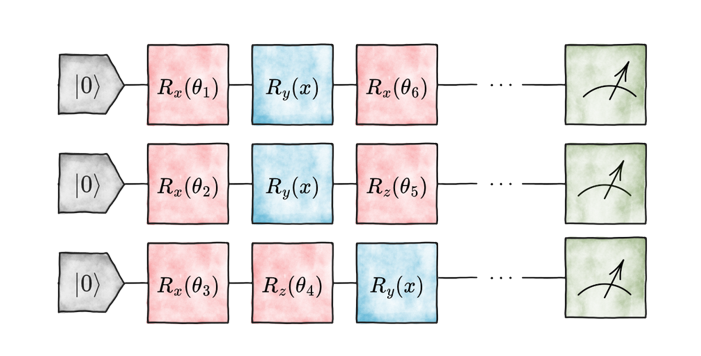
\includegraphics[width=0.9\textwidth]{figures/vqc.png}
  }
 \end{tabular}
 };
 
\node[state,
  right of = VQC,
  node distance = 3cm,
  yshift=2cm, 
  fill=blue!20] (NSHOT) 
 {\begin{tabular}{l}
 \textbf{Expected values}\\ 
 $y_{est} \equiv \braket{\psi'|\hat{O}|\psi'}$
  \end{tabular}
  };
 
\draw[line width=0.3mm] (1, -2.5)  to[out=0, in=200] (3, -3.2);
\draw[line width=0.3mm] (6, -2.8)  to[out=0, in=250] (7, -1.6);
\end{tikzpicture}

\end{frame}


% SLIDE 4 QML
\begin{frame}{Quantum Machine Learning}

\vspace{0.56cm}
\begin{tikzpicture}[->,>=stealth']

 \node[state, fill=orange!20] (ML) 
 {\begin{tabular}{l}
 \textbf{Machine Learning}\\ 
 \parbox{2.5cm}{$\mathcal{M}$: model;}\\
 \parbox{2.5cm}{$\mathcal{O}$: optimizer;}\\
 \parbox{2.5cm}{$\mathcal{J}$: loss function.}\\
 \parbox{2.5cm}{$(x, y)$: data}
  \end{tabular}
  };
  
  \node[state,
  below of = ML,
  yshift=-1.5cm, fill=blue!20] (QC) 
 {\begin{tabular}{l}
 \textbf{Quantum Computation}\\ 
 \parbox{2.5cm}{$\mathcal{Q}$: qubits;} \\
 \parbox{2.5cm}{$\mathcal{S}$: superposition;}\\
 \parbox{2.5cm}{$\mathcal{E}$: entanglement.}
  \end{tabular}
  };
  
 
 \node[state,
    right of=QC,
    yshift=-0.5cm,
    anchor=center,
    node distance=4.5cm, 	
    text width=3.5cm, fill=blue!20] (VQC) 
 {%
 \begin{tabular}{l}
  \textbf{Circuit execution} \\
  \parbox{4.5cm}{
  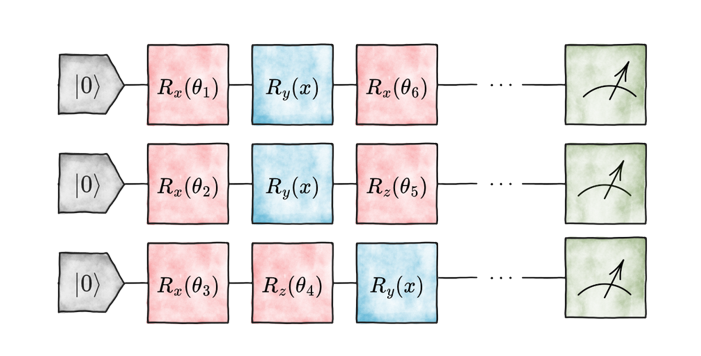
\includegraphics[width=0.9\textwidth]{figures/vqc.png}
  }
 \end{tabular}
 };
 
\node[state,
  right of = VQC,
  node distance = 3cm,
  yshift=2cm, 
  fill=blue!20] (NSHOT) 
 {\begin{tabular}{l}
 \textbf{Expected values}\\ 
 $y_{est} \equiv \braket{\psi'|\hat{O}|\psi'}$
  \end{tabular}
  };

  
 \draw[line width=0.3mm, red, opacity = 0.7] (0.5, 0.4)  to[out=0, in=230] (3, -3.3);
 \draw[line width=0.3mm, orange, opacity = 0.7] (-1.2, -1.25)  to[out=260, in=300] (4.4, -4.1);
 \draw[line width=0.3mm, cadmiumgreen, opacity = 0.7] (-0.4, -1.2)  to[out=330, in=80] (7.8, -0.4);
  
 
 \draw[red, line width=0.4mm, opacity = 0.9] (-1.1, 0.4) circle (0.4 cm);
 \draw[cadmiumgreen, line width=0.4mm, opacity = 0.9] (-0.65,-0.8) circle (0.3 cm);
 \draw[cadmiumgreen, line width=0.4mm, opacity = 0.9] (7.2,-1.4) rectangle (8.6, -0.95);
 \draw[orange, line width=0.4mm, opacity = 0.6] (-1.15,-0.8) circle (0.3 cm);
 \draw[red, line width=0.4mm, opacity = 0.6] (3.1,-4) rectangle (6,-2.4);
 \draw[orange, line width=0.4mm, opacity = 0.9] (3.5,-3.9) rectangle (5.2,-2.5);


\end{tikzpicture}
\end{frame}


% SLIDE 5 QML
\begin{frame}{Quantum Machine Learning!}

\vspace{0.42cm}
\begin{tikzpicture}[->,>=stealth']


 \node[state, fill=orange!20] (ML) 
 {\begin{tabular}{l}
 \textbf{Machine Learning}\\ 
 \parbox{2.5cm}{$\mathcal{M}$: model;}\\
 \parbox{2.5cm}{$\mathcal{O}$: optimizer;}\\
 \parbox{2.5cm}{$\mathcal{J}$: loss function.}\\
 \parbox{2.5cm}{$(x, y)$: data}
  \end{tabular}
  };
  
  \node[state,
  below of = ML,
  yshift=-1.5cm, fill=blue!20] (QC) 
 {\begin{tabular}{l}
 \textbf{Quantum Computation}\\ 
 \parbox{2.5cm}{$\mathcal{Q}$: qubits;} \\
 \parbox{2.5cm}{$\mathcal{S}$: superposition;}\\
 \parbox{2.5cm}{$\mathcal{E}$: entanglement.}
  \end{tabular}
  };
  

 \node[state,   
  text width=3cm, 
  yshift=1.5cm, 
  right of=ML, 	
  node distance=4cm, 
  anchor=center, fill=green!20] (OPT) 
 {%
 \begin{tabular}{l} 	% content
  \textbf{Optimizer $\mathcal{O}$}\\
  Hybrid-strategy
 \end{tabular}
 };
 
 \node[state,
    right of=QC,
    yshift=-0.5cm,
    anchor=center,
    node distance=4.5cm, 	
    text width=3.5cm, fill=blue!20] (VQC) 
 {%
 \begin{tabular}{l}
  \textbf{Circuit execution} \\
  \parbox{4.5cm}{
  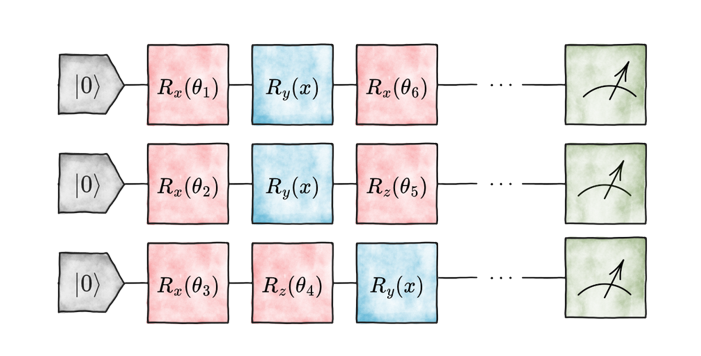
\includegraphics[width=0.9\textwidth]{figures/vqc.png}
  }
 \end{tabular}
 };
 
\node[state,
  right of = VQC,
  node distance = 3cm,
  yshift=2cm, 
  fill=blue!20] (NSHOT) 
 {\begin{tabular}{l}
 \textbf{Expected values}\\ 
 $y_{est} \equiv \braket{\psi'|\hat{O}|\psi'}$
  \end{tabular}
  };
  
  \node[state,
  above of = NSHOT,
  node distance = 1.5cm,
  yshift=0cm, fill=green!20] (J) 
 {\begin{tabular}{l}
 \textbf{loss function $\mathcal{J}$}\\ 
 $\mathcal{J}(y_{meas}, y_{est})$
  \end{tabular}
  };
  

 \draw[line width=0.3mm] (6.5, -3)  to[out=0, in=270] (7.5, -1.6);
 \draw[line width=0.3mm] (6, -1.1)  to[out=180, in=200] (6.1, 0.2);
 \draw[line width=0.3mm] (7.5, 1.1)  to[out=90, in=0] (5.7, 1.5);
 \draw[line width=0.6mm, opacity=0.8] (2, 1.6)  to[out=180, in=270] (-0.2, 2.9);
 
 \draw[line width=0.3mm, orange, opacity = 0.0] (-1.2, -1.25)  to[out=260, in=300] (4.4, -3.5);

\end{tikzpicture}
\end{frame}

\begin{frame}{From ML to QML}
\begin{figure}  
   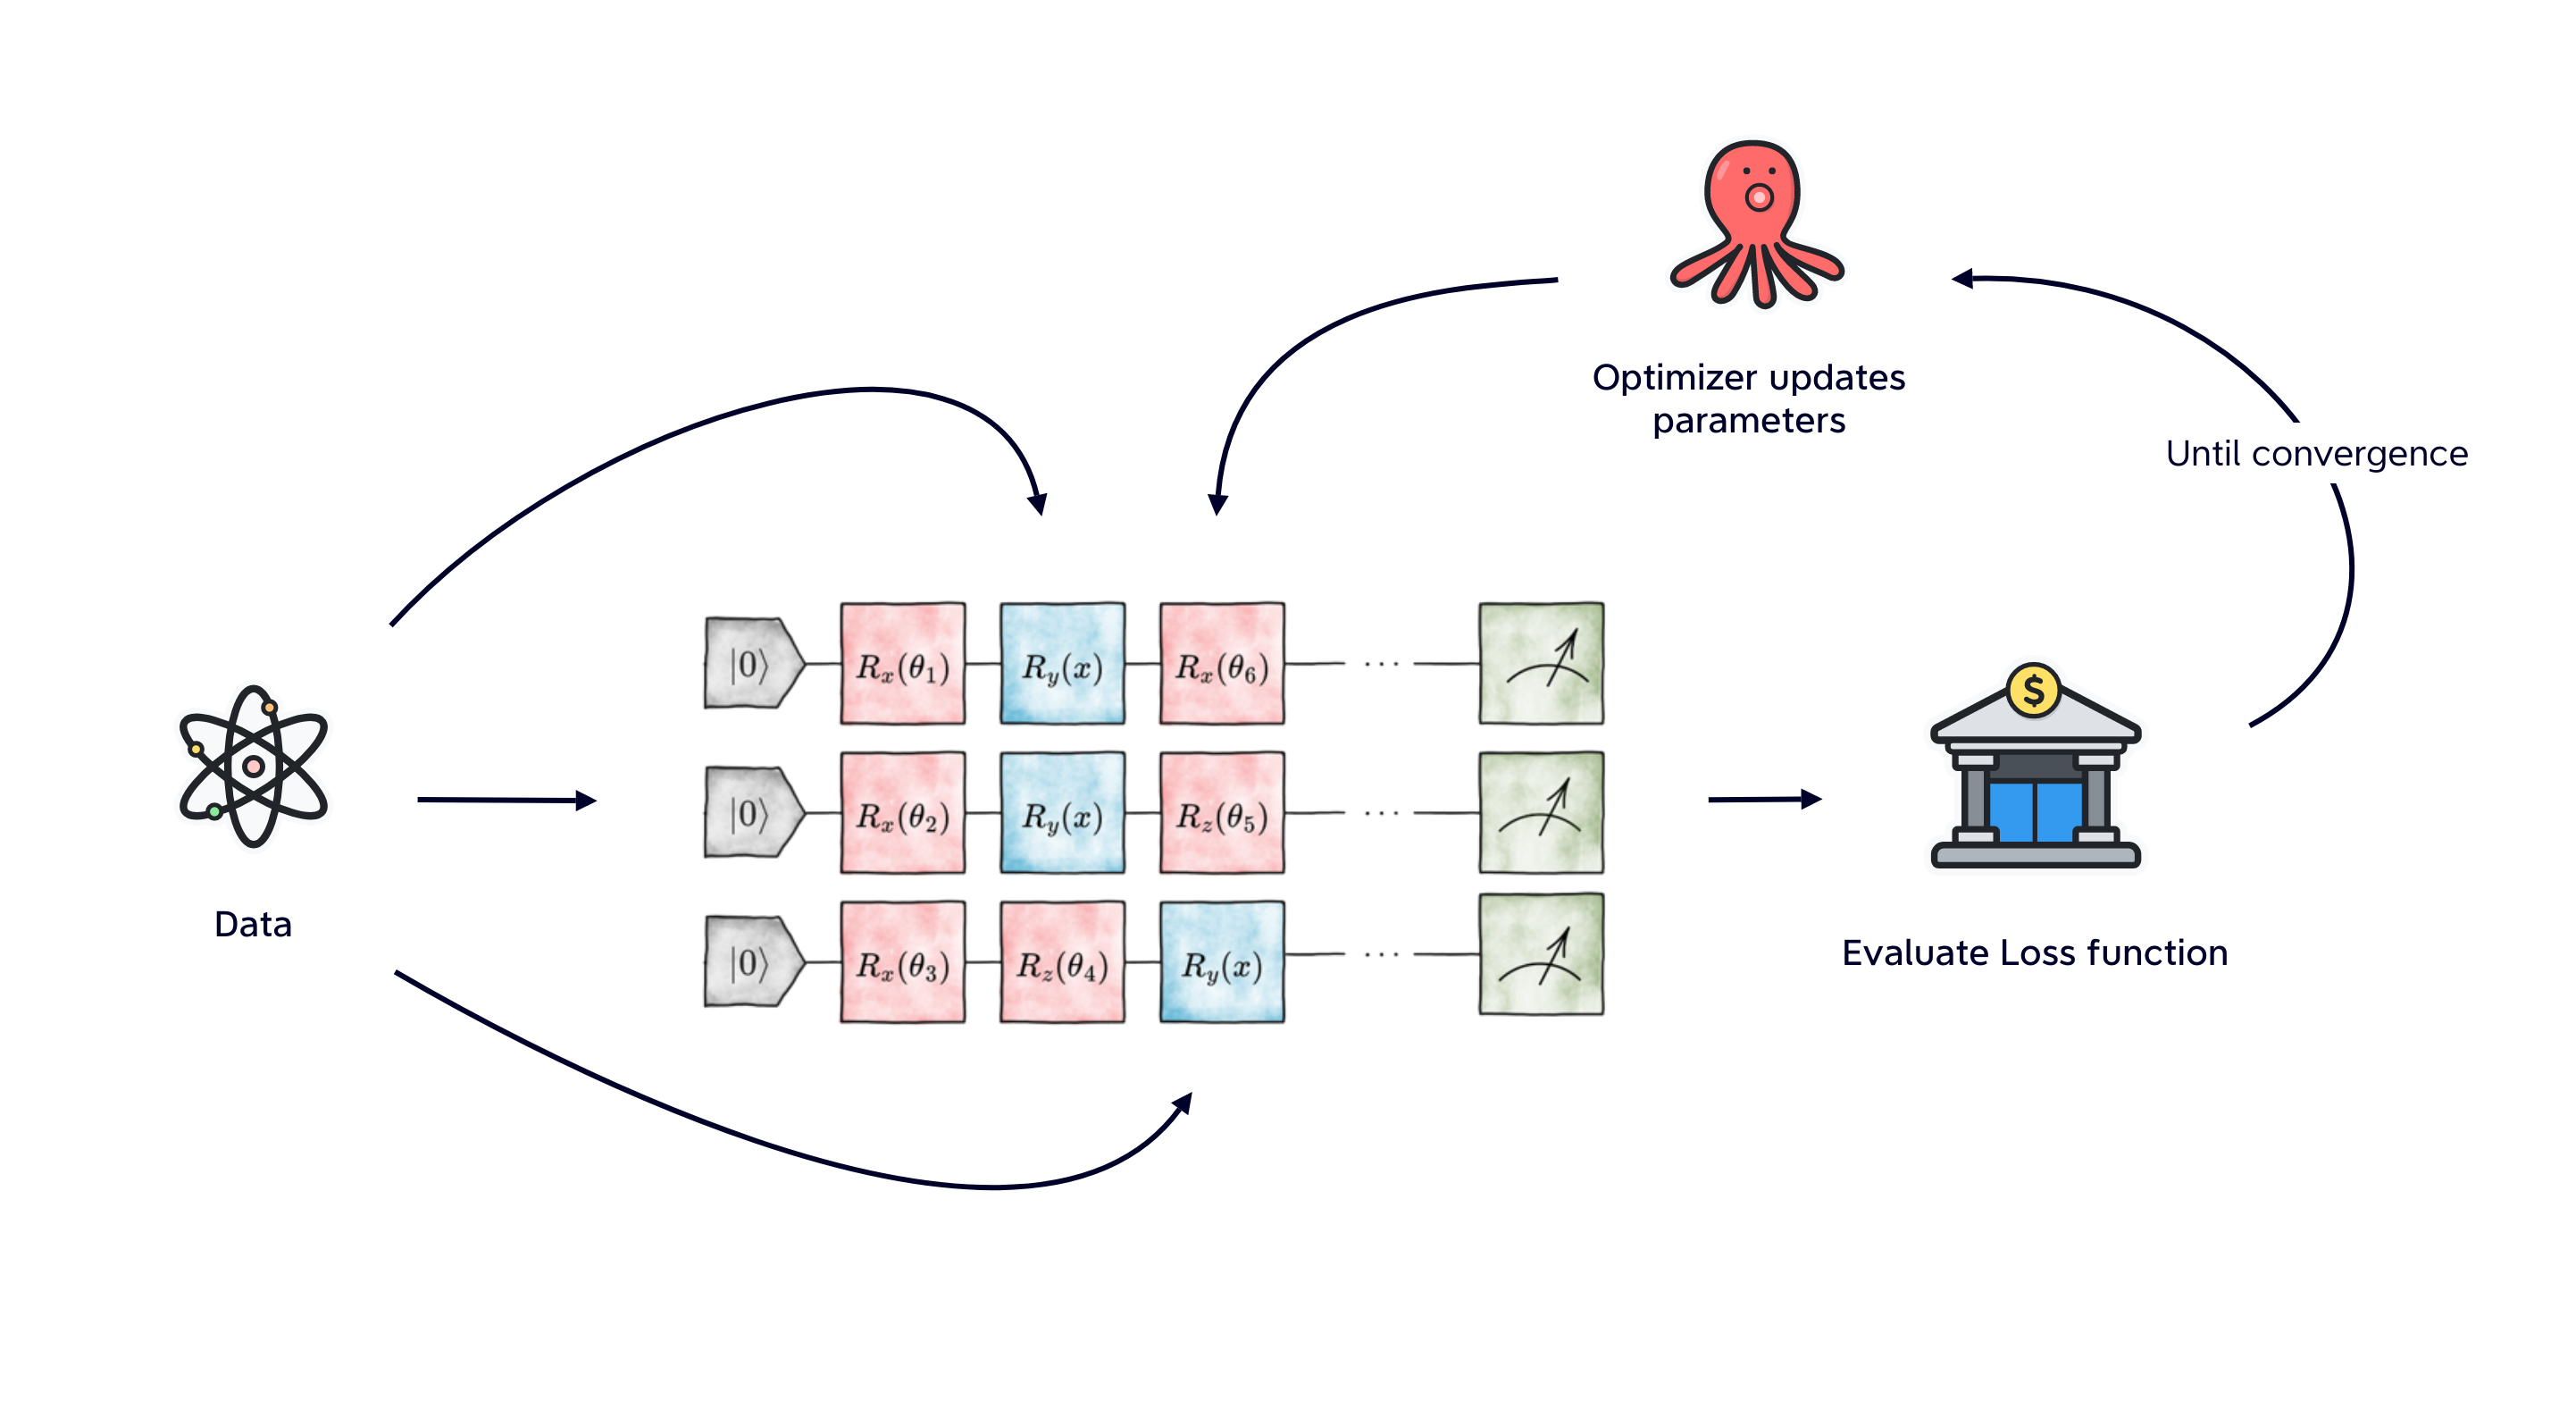
\includegraphics[width=1\textwidth]{figures/qml_scheme.png}
\end{figure}
\end{frame}

\begin{frame}{But can this work?}
\pause
\begin{itemize}[noitemsep]
\item[1.] Depend on the problem\pause, but what better of playing in the Hilbert space 
when tackling a many body system?
\pause
\item[2.] We can take some more rational proof of utility.
\end{itemize}
\pause
Using Variational Quantum Circuits we define a Variational Quantum Computer!
\pause
\begin{multicols}{2}
\begin{itemize}
\item<7,8,9>[1.] we want a quantum circuit $\mathcal{U}(\bm{\theta})$ to approximates some law $V$;
\item<8,9>[2.] executing $\mathcal{U}(\bm{\theta})$ we use a variational quantum state
to reach the solution;
\item<9>[3.] \textbf{Solovay-Kitaev theorem}: the number of gates needed by $\mathcal{U}$ to 
represent $V$ with precision $\delta$ is $\mathcal{O}(\log^c \delta^{-1})$, where
$c<4$.
\end{itemize}
\begin{figure}
    \uncover<6,7,8,9>{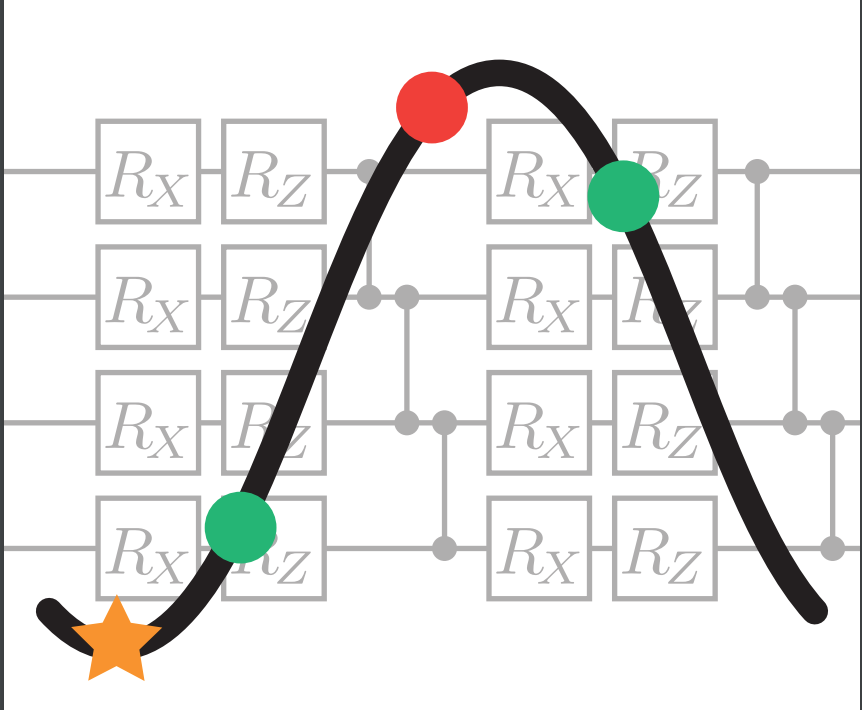
\includegraphics[width=0.5\textwidth]{figures/variational.png}}
\end{figure}
\end{multicols}
\end{frame}

\section{A practical example}

\begin{frame}{Approximating ground states - Adiabatic Computing}
\pause
What is a quantum annealer?
\pause
\begin{itemize}[noitemsep]
\item[\faLeaf] A QC with many spins arranged on a lattice connected to nearest neighbors;
\pause
\item[\faCrosshairs] typically Ising models can be encoded into a quantum annealer!
\pause
\end{itemize}
The game is to slowly (\textit{adiabatically}) move an $H_0$ to a target Hamiltonian $H_1$, in which we encode the problem:
\pause
 $$   H_{ad} = H_0 \bigl[1 - s(\tau)\bigr] + s(\tau) H_1. $$
 \vspace{0.3cm}
\pause
If adiabatic enough, you'll remain in the ground state.
\pause
\begin{multicols}{2}
\begin{figure}
    {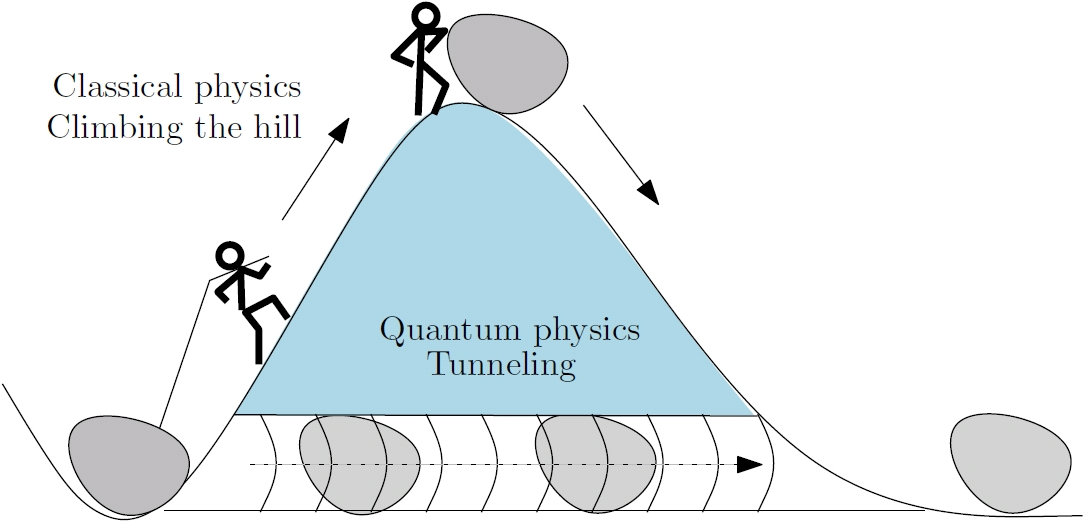
\includegraphics[width=0.47\textwidth, height=0.3\textheight]{figures/tunneling.png}
    \caption*{\href{https://arxiv.org/abs/2207.01827}{\faBook\,\,arXiv:2207.01827}}}%
    $\,\,$
    \pause
    {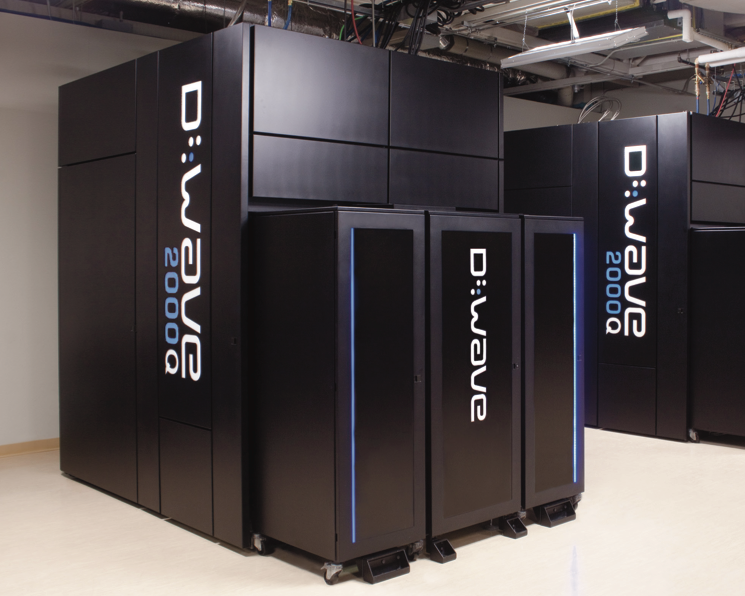
\includegraphics[width=0.4\textwidth, height=0.3\textheight]{figures/dwave.png}
    \caption*{\href{https://www.dwavesys.com/}{\faBook\,\,https://www.dwavesys.com/}}}%    
\end{figure}
\end{multicols}

\end{frame}

\begin{frame}{Approximating ground states - VQE \hfill \href{https://arxiv.org/abs/1304.3061}{\faBook\,\,arXiv:1304.3061}}
\pause
This method is known as Variational Quantum Eigensolver (VQE).
\pause
\begin{itemize}[noitemsep]
\item[1.] consider a target Hamiltonian $H_{\rm target}$, whose ground state is $\ket{\psi_0}$;
\pause
\item[2.] we take a parametrized quantum circuit $\mathcal{U}(\bm{\theta})$, with action $ \ket{q_f} = \mathcal{U}(\bm{\theta})\ket{0} $
\pause
\item[3.] the goal is to train $\mathcal{U}(\bm{\theta})$ to return a $\ket{q_f} = \ket{\tilde{\psi}_0}$.
\pause
\end{itemize}
\begin{figure}
    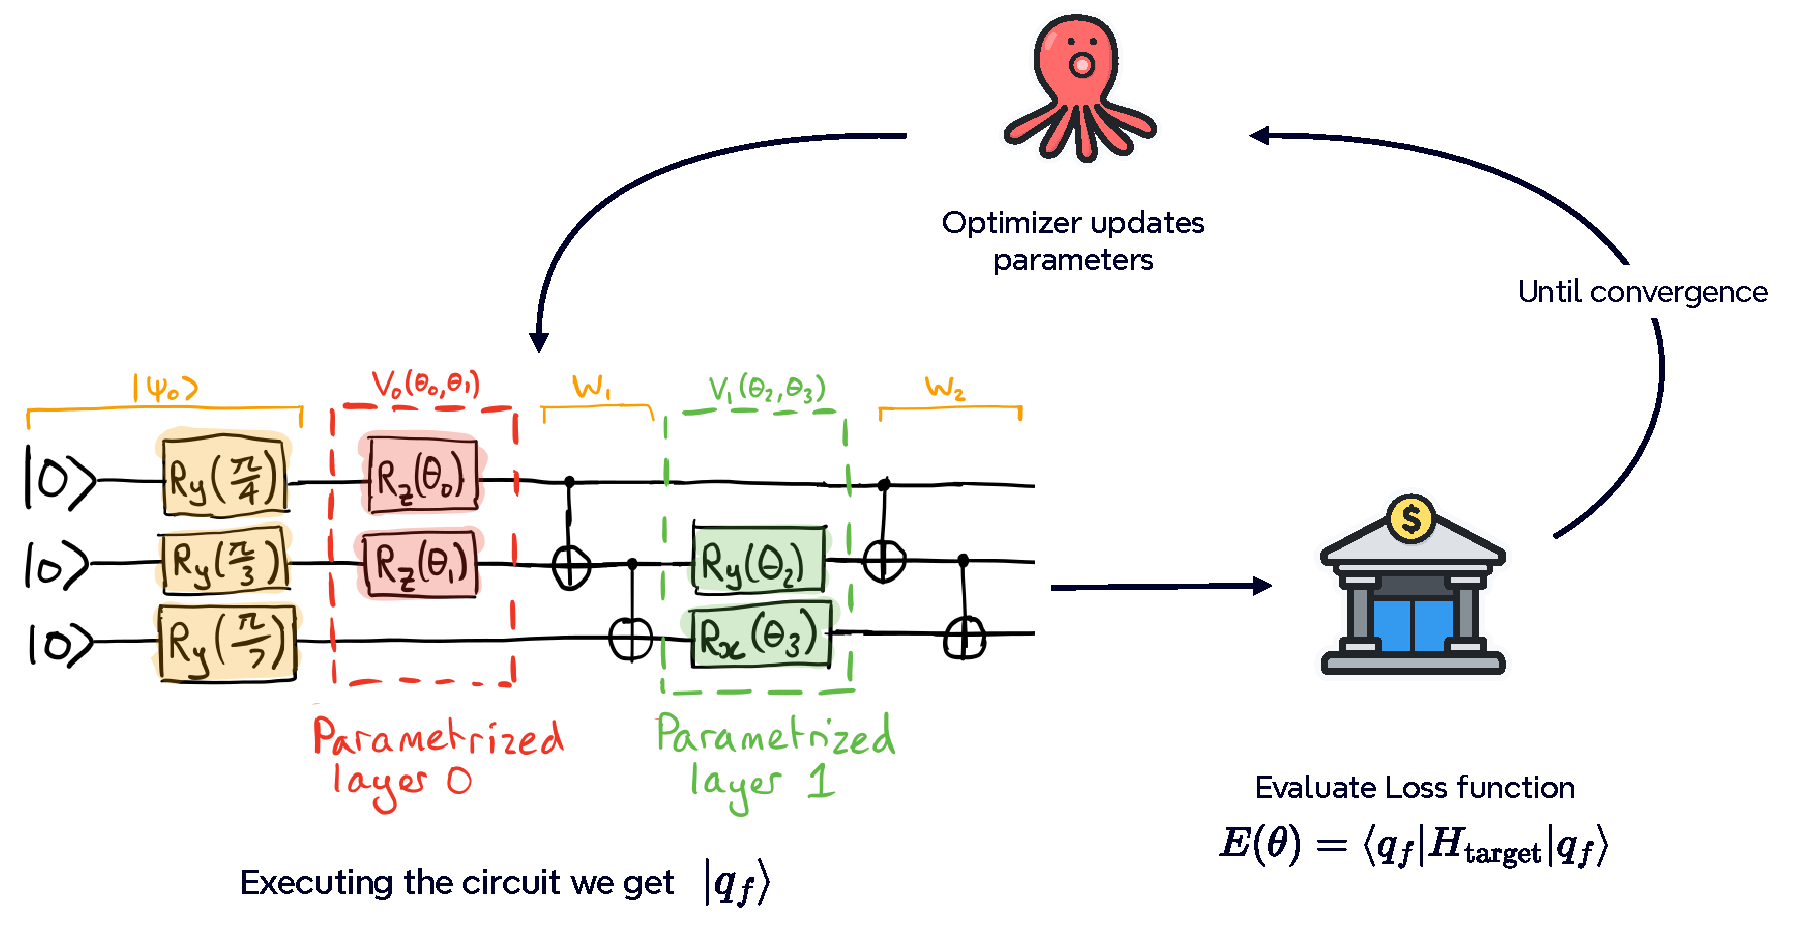
\includegraphics[width=0.9\textwidth]{figures/vqe.pdf}
\end{figure}
\pause
\begin{center}
\faTerminal\,\,Let's code it!
\end{center}
\end{frame}

\begin{frame}
\begin{figure}
    
\includegraphics[width=1\textwidth]{figures/thank.png}%
\end{figure}
\end{frame}

\end{document}
